%%!TEX encoding = UTF-8 Unicode
\documentclass[11pt,twoside,a4paper]{book}
\usepackage[czech, english]{babel}
\usepackage[T1]{fontenc}
\usepackage[utf8]{inputenc}
\usepackage{graphicx}
\usepackage{k336_thesis_macros}
\usepackage{listings}
\usepackage{textcomp}
\renewcommand{\ttdefault}{pcr}
\renewcommand{\lstlistingname}{Code Example}
\renewcommand{\lstlistlistingname}{List of Code Examples}
\let\Chapter\chapter
\def\chapter{\addtocontents{lol}{\protect\addvspace{10pt}}\Chapter}
\newcommand\TypeOfWork{Master's Thesis}   \typeout{Master's Thesis}
\newcommand\StudProgram{Electrical Engineering and Information Technology}
\newcommand\StudBranch{Computer Science and Engineering}
\newcommand\WorkTitle{Java implementation for Smalltalk/X VM}
\newcommand\FirstandFamilyName{Bc. Marcel Hlopko}
\newcommand\Supervisor{Ing. Jan Vraný PhD.}

\newcommand{\jv}[1]{{\color{red} #1}}
\newcommand{\libjava}{{Libjava}}
\newcommand{\jinterpret}{Jinterpret} 
\usepackage[
pdftitle={\WorkTitle},
pdfauthor={\FirstandFamilyName},
bookmarks=true,
colorlinks=true,
breaklinks=true,
urlcolor=red,
citecolor=blue,
linkcolor=blue,
unicode=true,
]
{hyperref}
\usepackage[square, numbers]{natbib}
\let\oldUrl\url
\renewcommand\url[1]{<\texttt{\oldUrl{#1}}>}

\lstdefinelanguage{Smalltalk}{ 
	morekeywords={true,false,self,super,nil, ifTrue, ifFalse, do, ifNotNil}, 
	sensitive=true, 
	morecomment=[s]{"}{"}, 
	morestring=[d]', 
	style=SmalltalkStyle 
} 

\lstdefinestyle{SmalltalkStyle}{ 
	literate={:=}{{$\gets$}}1{^}{{$\uparrow$}}1 
} 

\lstloadlanguages{C,Java,Smalltalk}

\lstset{
	morekeywords={OBJ},
	language=Smalltalk,
	numbers=left,
	numbersep=5pt,
	tabsize=4,
	captionpos=b,
	numberstyle=\tiny,
	frame=tb,
	columns=fixed,
	%basicstyle=\ttfamily\footnotesize,
	basicstyle=\ttfamily,
	extendedchars=true,
	framexleftmargin=17pt,
	framexrightmargin=5pt,
	framexbottommargin=4pt,
	xleftmargin=17pt,
	breaklines=true,
	keywordstyle=\bfseries,
	commentstyle=\textit
}


\begin{document}
\selectlanguage{english}
\typeout{************************************************}
\typeout{Language: english}
\typeout{Type of Work: \TypeOfWork}
\typeout{Study Program: \StudProgram}
\typeout{Study Branch: \StudBranch}
\typeout{Author: \FirstandFamilyName}
\typeout{Title: \WorkTitle}
\typeout{Supervisor: \Supervisor}
\typeout{***************************************************}
\newcommand\Department{Department of Computer Science and Engineering}
\newcommand\Faculty{Faculty of Electrical Engineering}
\newcommand\University{Czech Technical University in Prague}
\newcommand\labelSupervisor{Supervisor}
\newcommand\labelStudProgram{Study Programme}
\newcommand\labelStudBranch{Field of Study}
\coverpagestarts
\acknowledgements
\noindent
This thesis would not be possible without the help and leading of my supervisor, Jan Vraný.
Also, I would like to thank my parents for support and friends for patience and understanding, when they had to listen to me talking about the problems in this thesis.
\declaration{Prague, 1.\,12.\,2011}

\abstractpage

A possibility to compose program of multiple different programming languages
is becoming of great importance nowadays. For example, programmers can reuse
existing software libraries even if they are written in a different language,
which brings code use one level further. Recently, a lot of effort has been spent
on supporting multiple languages on both major runtime environments -- Java and CLR. 

In this thesis, we will describe an implementation of \libjava{}, a Java language implementation
running on top of Smalltalk/X virtual machine. Contrary to Java or CLR, \libjava{} is 
not translating Java programs into Smalltalk bytecode. Instead, the virtual machine was modified
so it can run both Smalltalk and Java bytecode. We have validated our implementation
on several large Java applications - JUnit testing framework, Groovy compiler, 
Eclipse Java Compiler and Apache Tomcat Servlet Container. 

\vglue30mm
\noindent{\Huge \textbf{Abstract}}

A possibility to compose program of multiple different programming languages
is becoming of great importance nowadays. For example, programmers can reuse
existing software libraries even if they are written in a different language,
which brings code use one level further. Recently, lot of effort has been spent
on supporting multiple languages both major runtime environemnts -- Java and CLR. 

In this thesis, we will describe an implementation of libjava, a Java language implementation
running on top of Smalltalk/X virtual machine. Contrary to Java or CLR, libjava is 
not translating Java programs into Smalltalk bytecode. Instead, the VM was modified
so it can run both Smalltalk and Java bytecode. We have validated our implementation
on several large Java applications - JUnit testing framework, Groovy compiler, 
Eclipse Java Compiler and Apache Tomcat Servlet Container. 

%%%%%%%%%%%%%%%%%%%%%%%%%%%%%%%%%%%%%%%%%%%%%%%%%%%%%%%%%%%%%%%%%%%%%%%%%%%%%%%%%%%%%%%%%

Lanugage interoperability problem is becoming very common in modern programming languages industry.
There are many languages written on top of existing Virtual Machines.
Smalltalk/X is Smalltalk implementation already having support for Ruby, Javascript, XQuery and Pascal. 
In this thesis we describe how we implemented support for Java programming language.
Our approach is unique in the way how we integrated Java into the Virtual Machine, making Smalltalk and Java equal.
We present solutions to encountered problems and validate our work on JUnit library, Groovy programming language written in Java and Tomcat, web application server for Java.

\vskip 2.75\baselineskip
\noindent

Une possibilité de composer le programme des langage différents multiples de programmation est de plus en plus grande importance de nos jours. 
Par exemple, les programmeurs peuvent réutiliser les bibliothèques logicielles existants même si elles sont écrites dans un langage différent, ce qui apporte l'utilisation du code de niveau plus haut.
Récemment, beaucoup d'effort a été dépensé sur le soutien des langages multiples sur les deux grandes runtime environnements Java Virtual Machine et CLR.

Dans cette thèse, nous allons décrire une mise en œuvre de \libjava{}, une implementation du langage Java qui s'exécute au dessus de Smalltalk/X machine virtuelle.
 Au contraire de langages fonctionnant sur JVM ou CLR, \libjava{} ne traduit pas des programmes de Java au bytecode de Smalltalk. 
Au lieu de cela, la machine virtuelle a été modifié de sorte qu'il peut fonctionner aussi bien Smalltalk que Java.
Nous avons validé notre mise en œuvre sur plusieurs applications Java grands - JUnit test framework, Groovy compilateur, le compilateur Java Eclipse et le serveur de servlet Apache Tomcat.

\tableofcontents
\listoffigures
\lstlistoflistings
\listoftables
\mainbodystarts
\normalfont
\parskip=0.2\baselineskip plus 0.2\baselineskip minus 0.1\baselineskip
\chapter{Introduction} 

A number of programming languages has been developed in the past and new ones are being developed. 
Although all general-purpose programming languages are in theory equivalent, in practice some languages better fit particular problem than another. 
Moreover, there is a lot of software libraries already written and possibility to reuse existing library greatly increases programmer's productivity. 

Recently, lot of effort has been done to support multiple languages. 
There is more than 300 languages implemented on top of JVM\cite{java-languages}.

\libjava{} is an implementation of Java language for Smalltalk/X environment. 
\libjava{} allows Java programs to run within Smalltalk/X environment. 
Smalltalk code can run Java code, which can in turn call back Smalltalk code. 
There were two main reasons for implementing Java in Smalltalk/X: 

\begin{itemize}
	\item reusing existing Java code in software written in Smalltalk/X
	\item being able to run Java code together with Smalltalk and other languages already supported by Smalltalk/X provides great vehicle for further research on language interoperability. 
\end{itemize}

A common approach chosen by both JVM and \href{http://msdn.microsoft.com/en-us/library/8bs2ecf4.aspx}{CLR} is to compile hosted languages into one intermediate language (Java bytecode in case of JVM or CIL in case of CLR).
The virtual machine understands and interprets this common intermediate representation.
However, such approach has few drawbacks. 
The main one is fact that the all features not directly supported by the common intermediate language must be emulated on top of it, which may be bit cumbersome and slow. 

On contrary to this traditional implementation, \libjava{} took different approach.
Instead of translating Java code into Smalltalk/X bytecode, the virtual machine has been modified so it can execute both Java and Smalltalk bytecodes. 
In other words, the virtual machine contains interpreter and compiler for both, Java and Smalltalk bytecode instructions. 

\section{Initial state}
We must say, that a lot of work has been done in past. 
Development of \libjava{} has been started by Claus Gittinger in 1996 and almost stopped in 1999, leaving \libjava{} being able to run Java applets using 1.1 runtime library. 
The basic architecture has been laid out by the original author. 

At the time, when we started working on \libjava{}, current version of Java was 1.6. 
\libjava{} was not able to start and run java programs using 1.6 runtime library. Many native method implementations were missing,some instruction semantic changed since then.  
Therefore, we had to implement missing features and fix some parts of the codebase that did not fit expected behavior. 
Following list summarizes changes and improvements we did:

\begin{enumerate}
	\item Changed native method binding mechanism
	\item Many native methods implemented
	\item Fixes in class loader
	\item Fixes in Java bytecode processor and decompiler
	\item Integration of \href{http://www.junit.org/}{JUnit} and \href{http://sourceware.org/mauve/}{Mauve} testing frameworks
	\item Redesigned Constant Pool content
	\item Reimplemented class resolving logic
	\item Implemented notion of Class Loader
	\item Class Space (JavaClassRegistry)
	\item Reimplemented synchronization (JavaMonitor) 
	\item Java support for stack unwind
	\item Constant Pool invalidation (unfinished)
	\item Java JIT compiler (unfinished)
\end{enumerate}

In following chapters, we will talk about how we designed and implemented new features, reasons, why we had to reimplement existing features and how we validated our result. 
In chapter \ref{chap:arch} we will familiarize the reader with general architecture, in chapter \ref{chap:loading} we will describe our class loading mechanism, in chapter \ref{chap:resolving} we will talk about new constant pool content and new resolving scheme. 
In chapter \ref{chap:monitors}, we describe how we achieved synchronization and locking across both Java and Smalltalk. 
Chapter \ref{chap:jit} deals with Just-in-Time compiler, our proposal on its behavior and review of current, not working implementation. 
Our testing approach is summarized in chapter \ref{chap:testing} and we validate the results in chapter \ref{chap:validation}. We summarize gained experience in chapter \ref{chap:summary}.

\section{Conventions}

Throughout the thesis, we will use conventions shown in Table \ref{tab:conventions}.

\begin{center}
	\begin{table}[ht]
		\centering
		\begin{tabular}{|l|p{7cm}|}
			\hline
			Example & Description \\
			\hline
			\hline
			\texttt{java.lang.Object} & Class names, inlined code \\
			\hline
			\texttt{JavaClassRegistry>>classForName:} & instance method classForName: of JavaClassRegistry class \\
			\hline
			\texttt{JavaVM class>>throwException:} & class method throwException: of JavaVM class \\
			\hline
			\texttt{Object\#toString()} & instance method toString() of Object class (notation for Java classes and methods) \\
			\hline
			\texttt{Double.parseDouble(String)} & static method parseDouble with one argument of type java.lang.String defined in class java.lang.Double \\
			\hline
		\end{tabular}
		\caption{Typing conventions}
		\label{tab:conventions}
	\end{table}
\end{center}


%*****************************************************************************
\chapter{Architecture}
\label{chap:arch}


\libjava{} itself consists of two parts: \textbf{VM support} consisting mainly of \textbf{Bytecode interpreter}, internally called \textbf{\jinterpret{}}, and \textbf{ST Runtime}, written in Smalltalk. 
In this chapter we will describe most important parts of \libjava{} and we will give the reader general understanding of how things work together and where a particular feature is implemented. 

\section{General Structure} 

\begin{figure}[ht]
	\begin{center}
		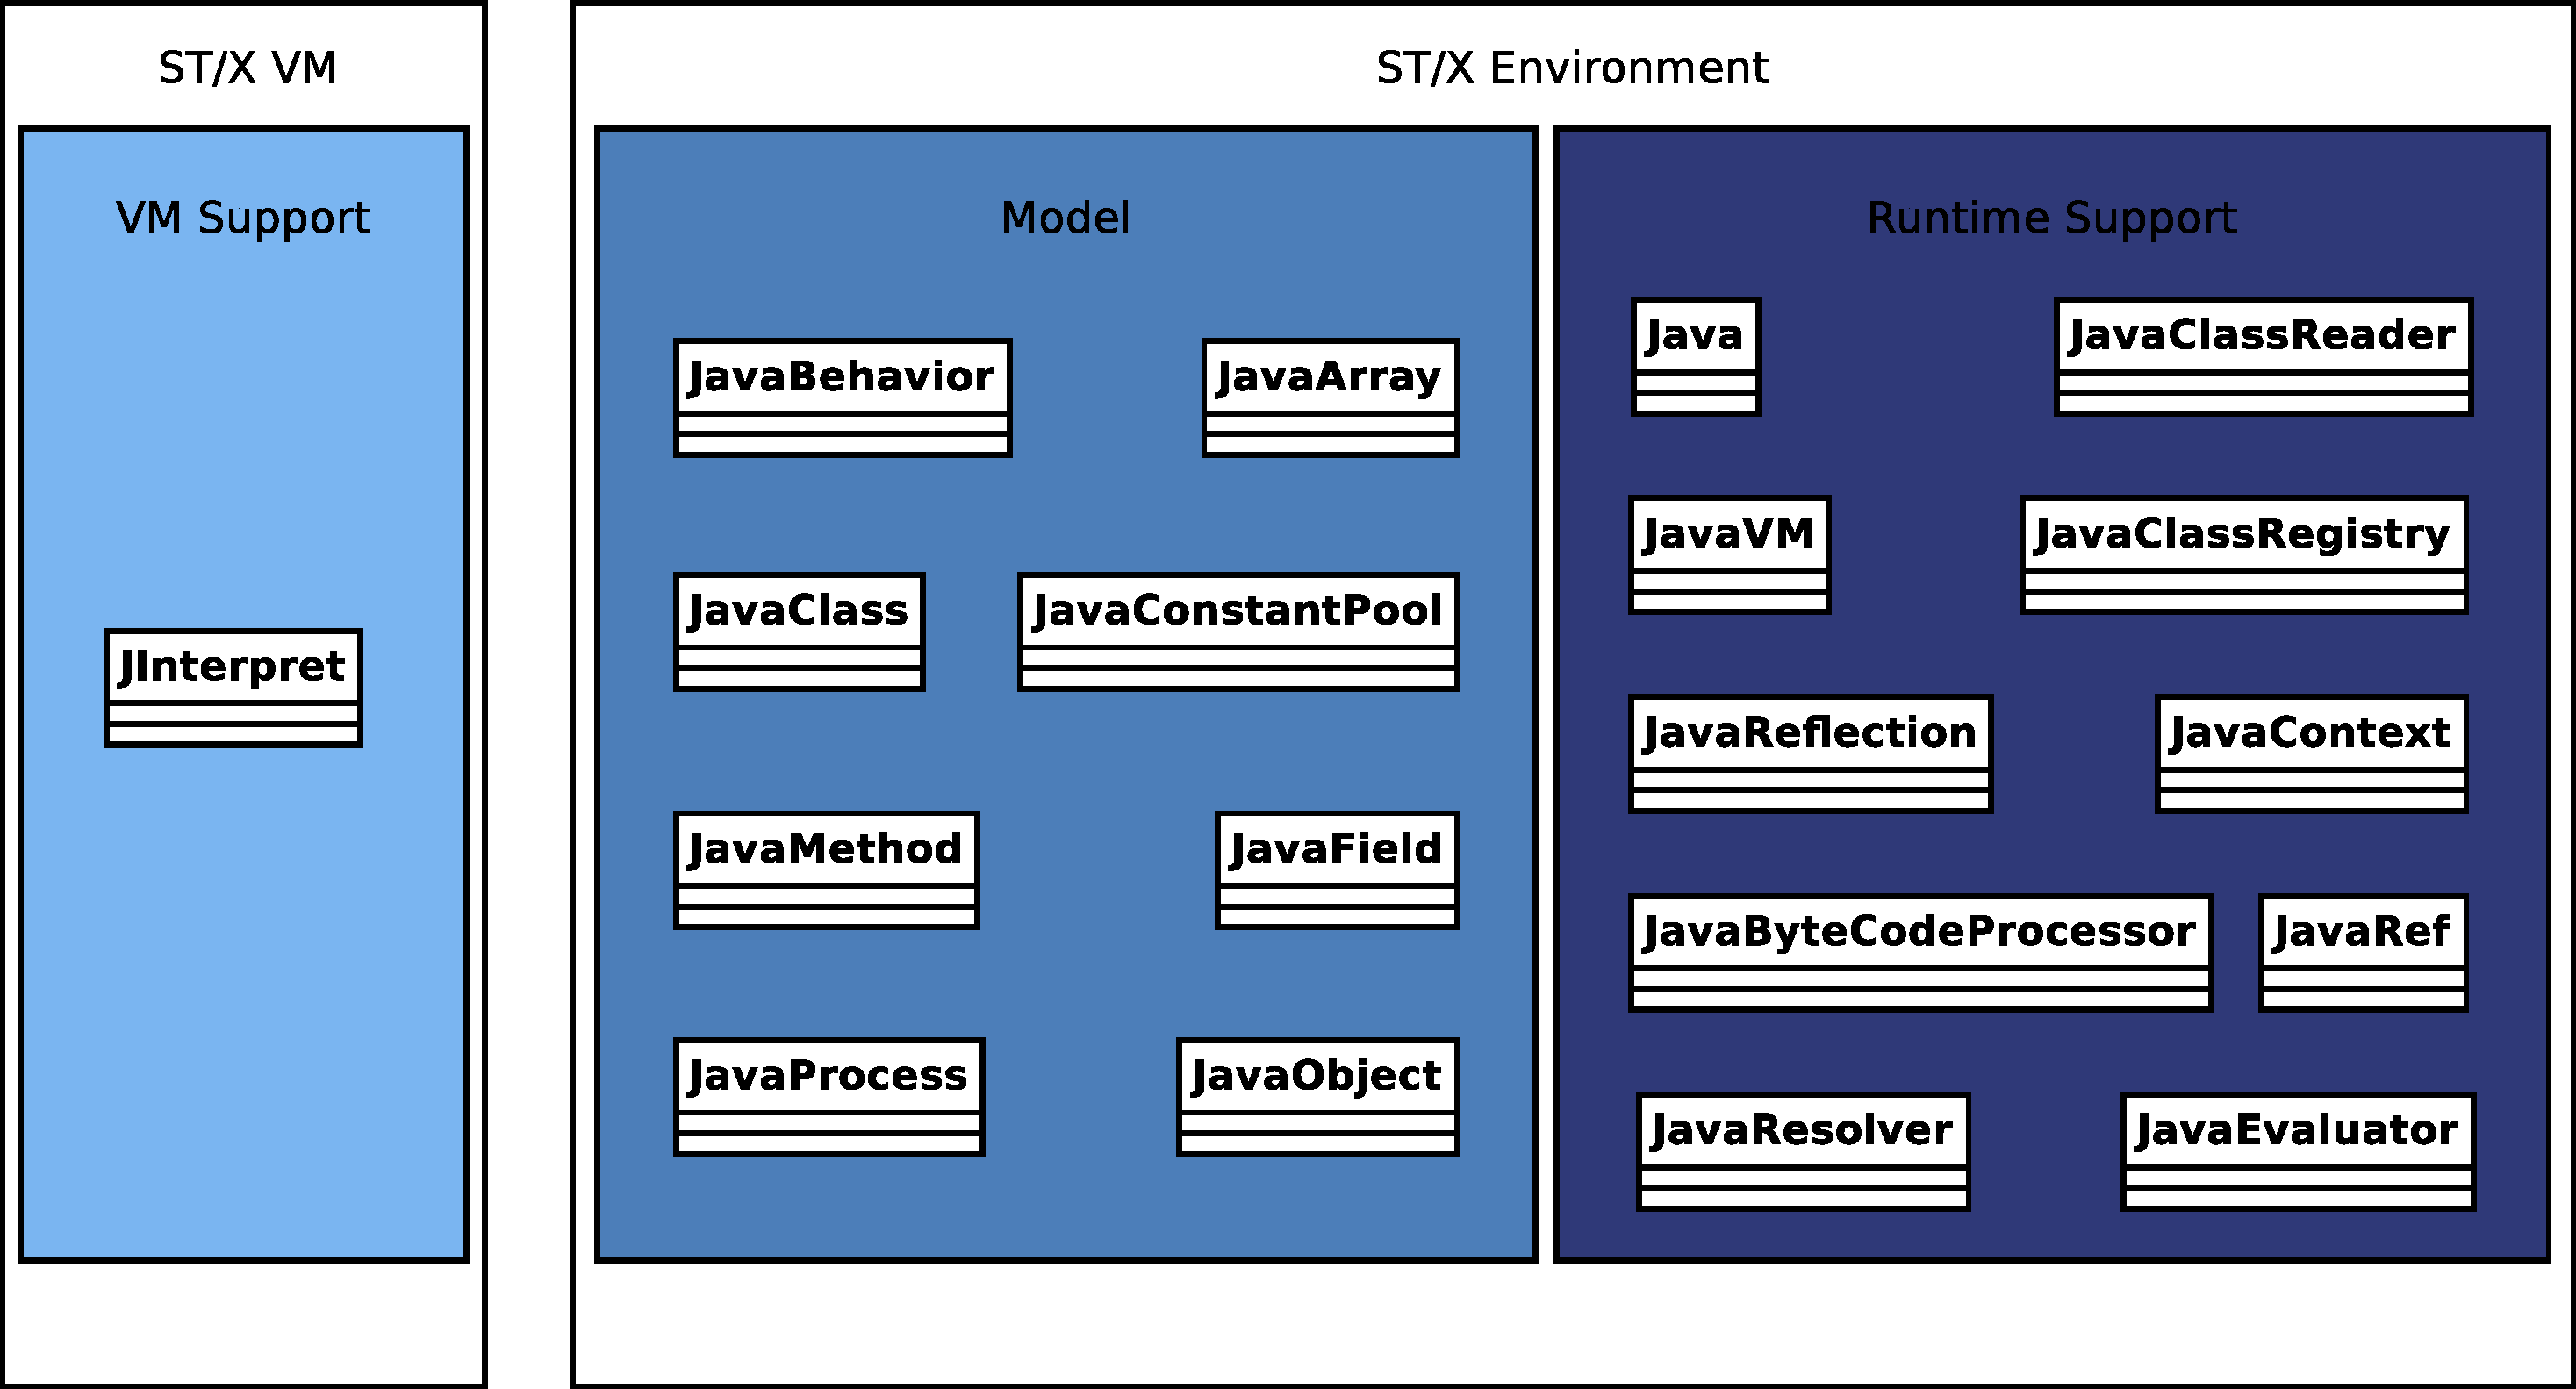
\includegraphics[width=15cm]{figures/libjava_world.pdf}
	\end{center}
	\caption{General structure of \libjava{}}
	\label{fig:libjava_world}
\end{figure}

Figure \ref{fig:libjava_world}, as mentioned, shows two parts. 
On the left side, virtual machine, on the right side, Smalltalk environment.
\textbf{Bytecode Interpreter} is written in C language as a part of ST/X virtual machine and the rest of \libjava{} is written in Smalltalk. 
Smalltalk part can be divided into \textbf{Model}, containing classes describing entities of Java language, such as \texttt{JavaClass} and \texttt{JavaMethod}. 
Mentioning these classes, it is important to note, that both Java class and Smalltalk class are first class citizens, they are both subclasses of common parent and they behave identically.
Similarly, Smalltalk and Java methods are both executable code, there is not an emulation involved.
\textbf{Runtime Support} consists of classes implementing logic livening up the model. 

\section{VM Support}

\libjava is not Java bytecode to Smalltalk bytecode compiler, it directly interprets Java bytecode.
Because of that, virtual machine support is needed, for performance reasons.

\subsection{Bytecode Interpreter}

Initial version of \libjava{} used Java interpreter written in C language. 
This interpreter is part of Smalltalk/X virtual machine. 
Interpreting Java in compiled C code is more effective than doing so in Smalltalk.

In order to support Bytecode Interpreter, ST/X virtual machine has been changed, so it is aware of Java methods.\footnote{More about Java methods can be seen in section \ref{sec:java_class}}
When a method is executed, VM checks if the method is defined in Smalltalk or Java, and handles the method appropriately. 
In case of Java method, interpretation is passed to Bytecode Interpreter. 
Bytecode Interpreter then creates instance of \texttt{JavaContext}, object representation of \textbf{stack frames} in Smalltalk, available to the running Smalltalk code and programmer. 
Bytecode Interpreter initializes context and starts executing method's bytecode. 


\subsection{Java Frame Representation}

Instances of class \texttt{JavaContext} represent activation records for all Java methods being executed within Smalltalk/X VM.
Java contexts are  created by the Bytecode Interpreter for each invoked method.
\texttt{JavaContext} extends \texttt{Context} (stack frame representation for Smalltalk methods) and adds some instance fields and methods to support Java language, namely:

\begin{itemize}
	\item Monitor support
	\item More than 16 method parameters support
	\item Exception handling
	\item Correct cleanup after unexpected termination (for example after thrown exception)
	\item Execution of \texttt{finally} blocks
\end{itemize}

\subsection{Native method invocation}

Java native methods are methods written in native code in the JVM itself or in a library linked to the JVM. 
Via native methods, Java code can access JVM internal state, hook and modify JVM behavior, access facilities outside the Java environment (such as operating system services) or profit from faster implementation. All native methods are marked as so using ACC\_NATIVE bit. 
When a Java native method is to be executed, Bytecode Interpreter recognizes it and sends \texttt{nativeMethodInvokation} to the method, as shown on \ref{code:native_method_invocation}.

\begin{lstlisting}[language=C, caption=Checking for and invocation of Java native method, label=code:native_method_invocation]
if (accessFlags & __MASKSMALLINT(__ACC_NATIVE)) {
    result = _SEND0(__aJavaMethod, 
        MKSYMBOL("nativeMethodInvokation"), nil, &nmi);
}
\end{lstlisting}

On the line 2, \texttt{if} condition is true if method has particular flag set.
Return value of \texttt{JavaMethod>>nativeMethodInvokation} is stored in \texttt{result} variable (line 3), which is later on
returned as a return value of the native method. 
\texttt{nativeMethodInvokation} method is responsible for looking up an implementation and execution of given native method. 
Its principal code is shown at Figure \ref{code:st_native_method_invocation}.

\begin{lstlisting}[caption=nativeMethodInvokation ST method, label=code:st_native_method_invocation]
nativeMethodInvokation
    | sel  mthd  sender |
    sel := self searchNativeImplementation.
    mthd := (JavaVM class compiledMethodAt: sel).
    sender := thisContext sender.
    ^ JavaVM perform: sel with: sender.
\end{lstlisting}

First, using method's selector, we search for corresponding method on \texttt{JavaVM class} (line 3).
Details of this method are shown at Figure \ref{code:st_search_native_implementation}.
On line 4, method object is retrieved from \texttt{JavaVM}.
On line 5, Java context, from which the method was invoked, is stored in \texttt{sender} variable.
Finally, on the line 5, method is performed, with current Java context as parameter.

\begin{lstlisting}[caption=searchNativeImplementation ST method, label=code:st_search_native_implementation]
searchNativeImplementation
    | name  selector |
    name := selector upTo: $(.
    selector := (
        '_' , 
        ((javaClass name copyReplaceAll: $/ with: $_) replaceAll: $$ with: $_) ,
        '_' , name , ':'
                ) asSymbol.
    (JavaVM class canUnderstand: selector) ifTrue: [
        ^ selector
    ].
    self compileNativeImplementationStub: selector.
    ^selector.
\end{lstlisting}

On Listing \ref{code:st_search_native_implementation}, implementation of \texttt{JavaMethod>>searchNativeImplementation} method is shown.
On line 2, methods name (without parentheses), is stored in \texttt{name} variable.
In \texttt{selector} variable, fully qualified Java method's name is transformed into valid ST selector (line 4).
For example, Smalltalk selector for \texttt{java.lang.Object\#wait()} is \texttt{\_java\_lang\_Object\_wait}.
If computed selector is already present in \texttt{JavaVM}, it's returned.
If not, a stub (method which just throws an exception) is compiled into \texttt{JavaVM}, and selector is returned (line 9 and 10).

There is roughly 900 shared native methods in \href{http://openjdk.java.net/}{OpenJDK}, plus around 700 unix specific. 
Altogether (shared, Linux, Solaris and Windows native methods), there is 2034 native methods, which should be implemented to have fully compliant implementation given that all features are implemented correctly.
At the time of writing this thesis, there were 705 already implemented in \libjava{}.
Writing native method implementations is time consuming, but rather straightforward task. 
Due to the time and resources constraints, we limit ourselves to implement only those needed by application or library we  would like to run.

\subsection{Implementing native methods}

If someone wanted to use native method in his Java program interpreted by \libjava{}, he can just execute the program.
When a native method is invoked, the debugger window will be opened, and the behavior of the method can be implemented there.
To each native method implementation in the \texttt{JavaVM} class, an instance of \texttt{JavaContext} is passed as argument,
holding all arguments passed to the native function. Example of implemented native method is shown on Listing \ref{code:native_method_example}.

\begin{lstlisting}[caption=Example of Java native method implementation, label=code:native_method_example]
_java_lang_Thread_interrupt0: nativeContext 
    | jThread  stProcess |

    jThread := nativeContext receiver.
    stProcess := self stProcessForJavaThread: jThread.
    stProcess javaInterrupt.
\end{lstlisting}

On the Listing \ref{code:native_method_example}, we can see implementation of the \texttt{java.lang.Thread\#interrupt0()} native method. 
On the line 1, transformed selector can be seen.
Receiver of the method (object, on which method was called) is assigned into \texttt{jThread} variable (line 4).
Next, corresponding instance of \texttt{Process} (Smalltalk class that represents a thread) is looked up and stored in \texttt{stProcess} variable.
Finally, \texttt{javaInterrupt} message is sent to the \texttt{stProcess} resulting in process interruption

\subsection{Instructions with complex semantics}

Vast majority of bytecode instructions are quite simple, such as \texttt{xCONST, xLOAD, xSTORE}, which just manipulate primitive data types, but there are few instructions, whose semantics is rather complex - \texttt{MONENTER, MONEXIT, ATHROW} or \texttt{CHECKCAST} for instance. 
When a more complex instruction is interpreted, Bytecode Interpreter can fall back to the Smalltalk code (in other words, call Smalltalk method, in most cases, on the \texttt{JavaVM} class).
Calling Smalltalk method from Bytecode Interpreter during interpretation brings certain overhead, but greatly eases implementation, debugging and testing and coding complex logic is time-consuming and error-prone. 

For most of such complex instructions, Smalltalk methods serve only as a trampoline for unhandled cases so the Smalltalk method
is actually executed rarely. Figure \ref{code:arraylength} shows an excerpt of \jinterpret{} implementation of an \texttt{ARRAYLENGTH} 
instruction. 

\begin{lstlisting}[language=C, caption=ARRAYLENGTH instruction, label=code:arraylength]
    case J_ARRAYLENGTH:
    {
        OBJ v;

        v = sp[-1];      /* array */
        if (__isArray(v)) {
            sp[-1] = __MKSMALLINT(__arraySize(v));
            break;
        }
        if (__isStringLike(v)) {
            sp[-1] = __MKSMALLINT(__stringSize(v));
            break;
        }
        if (__isByteArray(v)) {
            sp[-1] = __MKSMALLINT(__byteArraySize(v));
            break;
        }
        if (__isSignedIntegerArray(v)) {
            sp[-1] = __MKSMALLINT(__integerArraySize(v));
            break;
        }
        ...
        sp[-1] = _SEND1(JavaVM, MKSYMBOL("_ARRAYLENGTH:"), nil, &dummy1, v);
        ...
    }
    break;
\end{lstlisting}

\texttt{If} branches on lines 6, 10, 14, 18 are handling cases for a particular argument passed to \texttt{ARRAYLENGTH}.
If one of these cases occur, return value is pushed onto the stack, Smalltalk method is not invoked.
But if argument passed to \texttt{ARRAYLENGTH} does not fall into any of these cases, handling is delegated to \texttt{JavaVM class>>\_ARRAYLENGTH:} method (line 23).
\texttt{\_SEND1} macro is used, which represents a method send with one argument.

\subsection{Supporting more than 16 method arguments}
\label{sec:many-arguments}

Current Smalltalk/X VM supports up to 16 method arguments, i.e., it cannot handle method with more than 16 arguments. However, JLS defines, that Java can have up to 255 arguments.\cite[section~4.3.3]{jls}
To support methods with too many arguments, Java method with too many arguments is marked by a flag.
When a Java method is executed, the flag is checked.
If it is set, Bytecode Interpreter expects arguments to be passed in as array.
Bytecode Interpreter then unpacks the array and stores arguments into the Java context.

\section{Java Class Model}

Smalltalk and Java are both falling into category Class-based, Object-Oriented languages.
However, both embrace Object Orientation from slightly different angle. 

\subsection{Smalltalk Object Model}

Smalltalk/X, as every smalltalk system following heritage of Smalltalk-80 defined by \textbf{Smalltalk-80: Language and its implementation} book\cite{bluebook}, has uniform object model (Figure \ref{fig:st_object_model}).

\begin{enumerate}
	\item Everything is an object
	\item Every object is instance of a class, which is also and object
	\item Each class is inheriting its behavior from a single superclass
	\item Objects only communicate only via message passing
\end{enumerate}


\begin{figure}[ht]
	\begin{center}
		\includegraphics[width=14cm]{figures/smalltalk_object_model.pdf}
	\end{center}
	\caption{Smalltalk Object Model}
	\label{fig:st_object_model}
\end{figure}

One object can access state of another object only via messages, accessing other object's data is not possible. 
Because every object is instance of a class, even the class itself, method lookup algorithm is straightforward - when an object receives a message, corresponding method is looked up in object's class. 
If method is not found, searching continues in class' superclass. 
Lookup ends, when \texttt{nil} is searched, \texttt{nil} is superclass of \texttt{Object}.

\subsection{Java Object Model}

Java Object model is shown on Figure \ref{fig:java_object_model}. 
It's necessary to say that not everything in Java is an object, Java has primitive types such as \textbf{int} and \textbf{char}, a special constant \textbf{null}, and one built-in type - \textbf{String}, which is an object type, but language syntax allows for literal representation of strings. 
Special place has \textbf{null}, which is, on contrary to Smalltalk, not an object.
Java classes are not first class objects, they live in JVM in a separate memory area. 
Class can be accessed via \texttt{getClass()} method, which returns a \textbf{mirror} to the internal class representation.\cite{mirrors}
A root of a class hierarchy in Java is \texttt{java.lang.Object}. 
Every object in Java is instance of a class. 
Every class has superclass, except of \texttt{java.lang.Object} class whose superclass is  \textbf{null}. 

\begin{figure}[ht]
	\begin{center}
		\includegraphics[width=10cm]{figures/java_object_model.pdf}
	\end{center}
	\caption{Java Object Model}
	\label{fig:java_object_model}
\end{figure}

Java introduces notion of \textbf{static} fields and methods. 
Static field or method is shared among all instances of given class. 
Smalltalk alternatives are class fields and methods, but they have a different semantics.\footnote{Class methods in Smalltalk are inherited by subclasses (if not overridden)}
As an example of consequences of this design, method lookup algorithm for static and normal methods differ.

To avoid ambiguity, there cannot be two methods or fields with the same name in one class.
Subclass can override method or field, and it does not matter whether the overridden is static or not.

If the receiver is Java class, static method or field is looked up. 
If the current class does not have method (or field) with given name, search continues in a superclass.
Lookup ends after reaching \texttt{java.lang.Object}.

If the receiver is instance, method or field is looked up in instance and static methods (or fields). 
If not found, the same happens in superclass until reaching \texttt{java.lang.Object}.
}

\subsection{Object Model Mapping}

Since \libjava{} is shares VM mechanism to execute Java code with Smalltalk, it must map Java code to Smalltalk classes.
Java classes have to be mapped to Smalltalk classes, Java methods have to be mapped to Smalltalk methods, etc.

Mapping of Java object model to Smalltalk is shown on Figure \ref{fig:obj_model_mapping}. 
\texttt{JavaObject} is root of Java hierarchy, with \texttt{java.lang.Object} being subclass of it. 
We introduced \texttt{JavaClass} as superclass of all Java classes. 
Each Java object is instance of \texttt{JavaObject} and has one instance of \texttt{JavaClass} associated with it as its \texttt{javaClass}. 
Each Java Class is instance of \texttt{JavaClass} and has one instance of \texttt{JavaClass} associated with it as its superclass.

\begin{figure}[ht]
	\begin{center}
		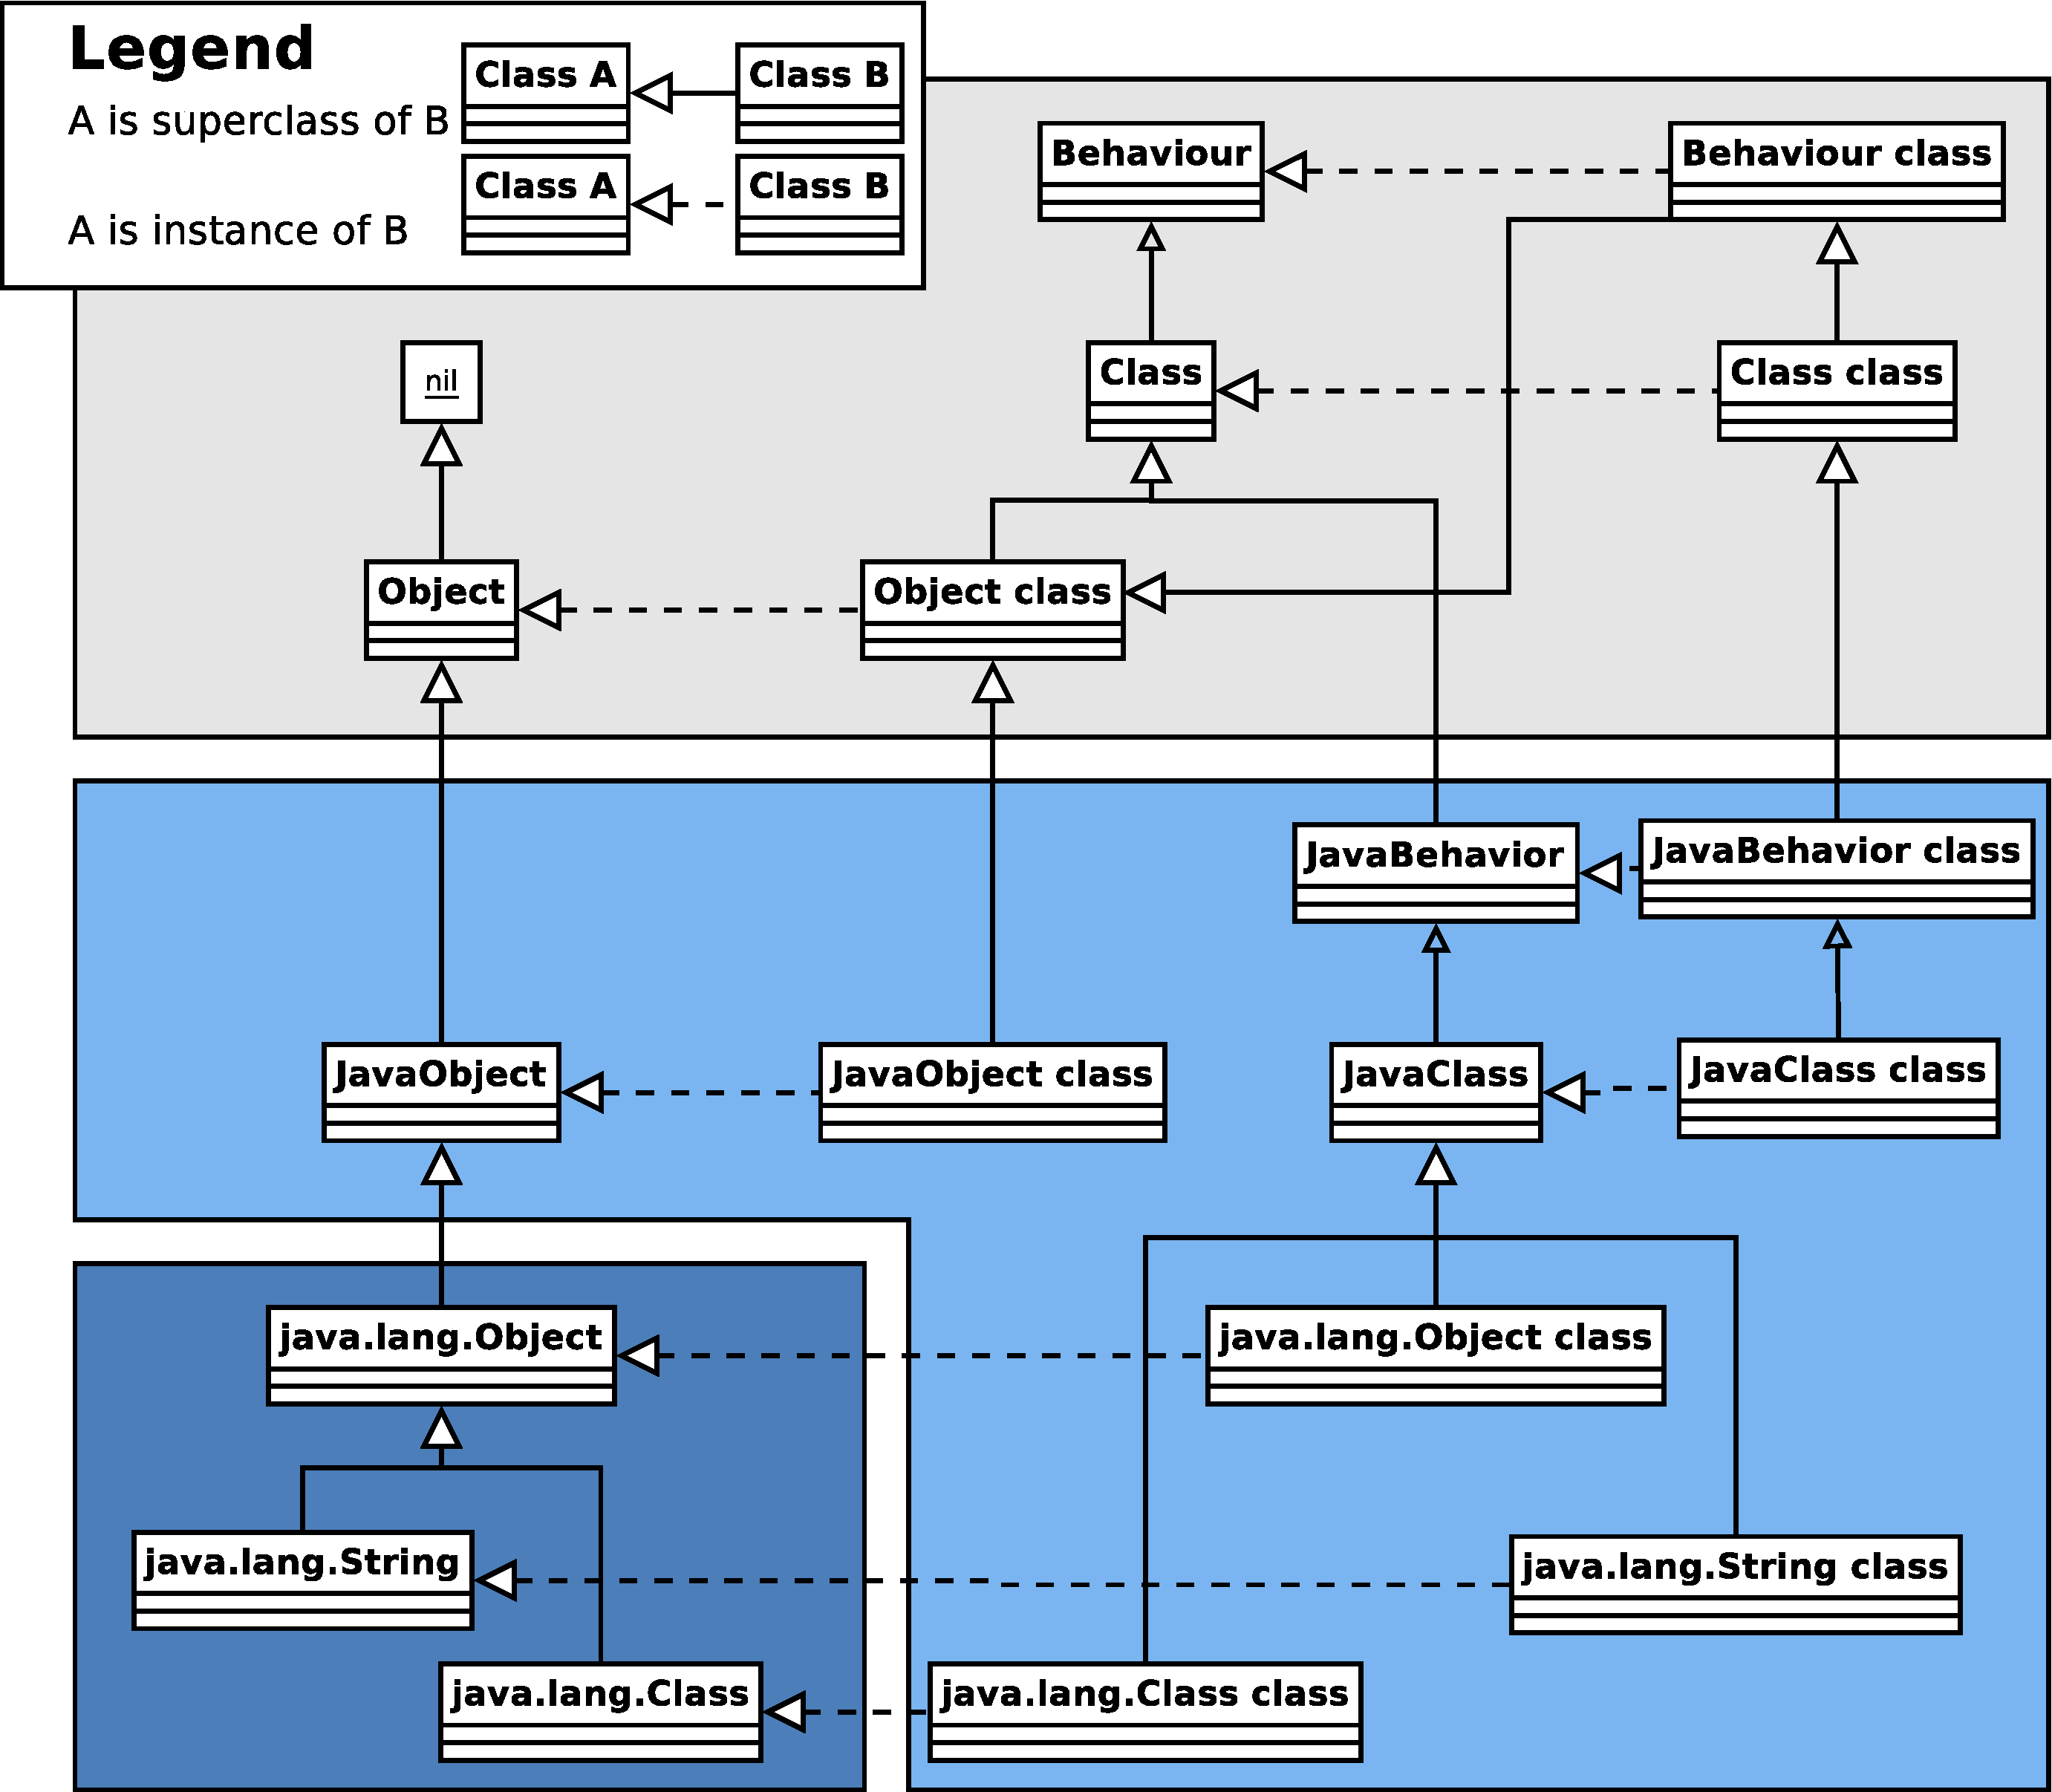
\includegraphics[width=12cm]{figures/object_model_mapping.pdf}
	\end{center}
	\caption{Java to Smalltalk Object Model Mapping}
	\label{fig:obj_model_mapping}
\end{figure}


\section{Runtime Support} 
\jv{explain!!! what is runtime support}

In this section we will describe the most important classes forming the \libjava{} runtime support. 
Runtime support classes in many ways simulate a work, which is normally done by JVM, some of them provide services to the programmer (such as \texttt{Java} class), some of them are important in connecting Java model classes together (such as \texttt{JavaClassReader}), etc.

\subsection{Java}

\texttt{Java} class is facade to the Java world inside Smalltalk. 
\texttt{Java} class provides following services:

\begin{itemize}
	\item Class loading and class access
	\item Java release access
	\item System properties
	\item Threads management
	\item Java initialization and teardown
	\item Java/Smalltalk object conversions
\end{itemize}

Two most important methods in \texttt{Java} class are \texttt{Java class>>~initializeJava}, which starts whole Java system, and \texttt{Java class>>flushAllJavaResources}, which will stop and clean up after running Java system.
Another interesting methods are \texttt{Java class>>classNamed:} and \texttt{Java class>>classForName:}.
First method will return already loaded Java class, or nil.
Second method will in case of not loaded class search classpath and load given class.

\subsection{JavaVM}

Runtime support and environment for Java. 
End user should not need to communicate with JavaVM directly, Java class should be used instead. 
\texttt{JavaVM} is layer between the native interpret and the rest of the system. 
\texttt{JavaVM} implements native methods invoked by interpret.
A list of services provided follows:

\begin{itemize}
	\item Class registry access
	\item Reflection
	\item Setting up default system properties
	\item Bytecode Interpreter complex instructions implementation
	\item Exceptions
	\item Synchronization, monitors
	\item Native methods implementation
\end{itemize}

\subsubsection{JavaClassRegistry}

JVM supports dynamic class loading using \textbf{ClassLoaders}. 
Basic principles and design reasons are pursued in \cite{bracha98}. 
JavaClassRegistry is class responsible keeping track of classes loaded by individual class loaders.
Class loading problems are rather subtle and we will offer our solutions to the reader in chapter \ref{chap:loading}.

\subsubsection{JavaReflection}

\texttt{JavaReflection} serves as a mirror allowing us to convert Java classes into their Smalltalk alternatives and vice-versa. 
When in Smalltalk, regular instances of \texttt{JavaClass} are used. 
But when a Java code for example calls \texttt{getClass()} or \texttt{String.class}, we need to convert Smalltalk class into the instance of \texttt{java.lang.Class}. 
This is done in \texttt{JavaReflection} class, also for arrays, objects, constant pools, methods, constructors, fields and strings.

\subsection{JavaResolver, JavaRef and subclasses}

In Java classfile, all references outside the classfile itself such as references to used classes, implemented interfaces and so on, are symbolic.\cite[chapter~4]{vmspec}
Such symbolic reference is represented by the \texttt{JavaRef} class and its subclasses. 
Symbolic references are stored in the \textbf{Constant Pool}.

Many instructions access constant pool content, for example \texttt{INVOKEx} instructions are given an index to the constant pool on which a method reference is stored.
This method reference is then resolved and method is invoked.

\texttt{JavaRef} is root of the Java reference hierarchy, it defines interface and structure accessed by Bytecode Interpreter. 
Together with primitive constants and \texttt{JavaNameAndType} are the only objects fount in \texttt{JavaConstantPool}. 
\texttt{JavaRef} descendant tree is quite big and consists of classes such as \texttt{JavaStringRef}, \texttt{JavaClassRef} or \texttt{JavaMethodRef}. 

We will deal with classfile reading and loading in chapter \ref{chap:loading}.

%*****************************************************************************
\chapter{Class loading}
\label{chap:loading}

Class loading is a process of loading new class from an external source, usually file, dynamically during runtime.
In this chapter, we will start with brief introduction into \textbf{Classfile} structure (\ref{sec:classfile}), followed by a closer look into \texttt{JavaClass} and its content (\ref{sec:java_class}).
Constant pool content is presented in \ref{sec:constant_pool}.
And at the end we present our findings and solutions regarding the \textbf{Class Loaders} issues (\ref{sec:class_loaders}).

\section{Classfile}
\label{sec:classfile}

Java classes are compiled by Java compiler into so called \textbf{Classfile}. Classfile format is specified by Java Language Reference.\cite[chapter~4]{vmspec} Basic classfile structure is shown in table \ref{tab:classfile}.

\begin{table}
	\centering
	\begin{tabular}{|l|p{11cm}|}
		\hline
		Section & Description \\
		\hline
		\hline
		Magic Number & Each classfile has to start with bytes \textbf{0xCAFEBABE} \\
		\hline
		Version & Major and Minor version numbers of the classfile. Java 6 has 50.0. \\
		\hline
		Constant Pool & Pool of constants referenced in the classfile \\
		\hline
		Access Flags & Denotes whether given class is public, abstract etc. \\
		\hline
		This Class & Name of this class \\
		\hline
		Super Class & Name of the superclass of this class \\
		\hline
		Interfaces & Enumeration of interfaces implemented by this class\\
		\hline
		Fields & Enumeration of all static and instance fields in the class\\
		\hline
		Methods & Enumeration of all static and instance methods in the class\\
		\hline
		Attributes & Supplementary attributes of the class, for example source file, annotations etc.\\
		\hline
	\end{tabular}
	\caption{Classfile structure}
	\label{tab:classfile}
\end{table}

We will not describe classfile format in more detail and will advise keen reader on the Java Language Specification \cite{vmspec}. 
For our purposes it is enough to know that classfile contains everything Java class needs to know to be able to be loaded and linked with running system. 
Constant pool is of great importance, describing references to the outside of the given class, which needs to be resolved in order to access runtime class, method, field or String representations of JVM.

\section{JavaBehavior, JavaClass and their content}
\label{sec:java_class}

Java class in our environment is represented by \texttt{JavaClass} class (\ref{fig:java_class}).
\texttt{JavaBehavior}, its direct superclass, is responsible for handling constant pool, access flags and interfaces.
It is subclass of \texttt{Class} class (representing Smalltalk class), inheriting for example notion of superclass and many more. 
Bytecode Interpreter is aware of \texttt{JavaBehavior} structure and directly accesses it.\footnote{Which means user can add fields to the \texttt{JavaClass}, but not to the \texttt{JavaBehavior}, without changing VM.} 

\texttt{JavaClass} implements the rest of features, which are not directly needed in Bytecode Interpreter and is open for extension.
To mention few of features \texttt{JavaClass} implements, there is class loader awareness, annotations, static fields or protection domain.

Instance and static fields are represented by \texttt{JavaField}.
Instances of JavaField know their index into instVars array of Java object. 

\texttt{JavaMethod} represents a Java method. Each class has its methods stored in its method dictionary, just like Smalltalk classes have. 
\texttt{JavaMethod} is subclass of \texttt{CompiledCode}, which is a common superclass representing bytecode-compiled executable thingy.
This allows us to use Java methods just like any other Smalltalk method and eases integration of Java methods into development tools. 
JavaMethod has three subclasses, \texttt{JavaMethodWithException}, representing any Java method, which declares throws clause, \texttt{JavaMethodWithHandler}, representing Java method, which has catch block in its body, and \texttt{JavaNativeMethod}, which represents method written in native code. 

\begin{figure}[ht]
	\begin{center}
		\includegraphics[width=15cm]{figures/java_class.pdf}
	\end{center}
	\caption{JavaClass}
	\label{fig:java_class}
\end{figure}

\section{Constant pool content}
\label{sec:constant_pool}

Constant pool is a structure where all constants from classfile are stored - integers or UTF8 literals, but also class references, method references, or field references. 
Because runtime system during compilation can differ from the system used to load class file and execute the code, all references to the outside of the class must be symbolic and must be resolved in run time.\footnote{Or at load time, we will talk about reasons for first or second way in chapter \ref{chap:resolving}} 
Figure \ref{fig:cp_content} shows classes, instances of which can be found in runtime constant pool of Java class.
Besides them, there are only primitive values, such as numbers or strings.

\begin{figure}[ht]
	\begin{center}
		\includegraphics[width=12cm]{figures/cp_content.pdf}
	\end{center}
	\caption{Constant pool content}
	\label{fig:cp_content}
\end{figure}

We shortly describe each of these classes in the Table \ref{tab:cp_content}.

\begin{table}[ht]
	\centering
	\begin{tabular}{|l|p{10cm}|}
		\hline
		Class & Description \\
		\hline
		\hline
		\texttt{JavaRef} & Root class defining interface with no functionality. \\
		\hline
		\texttt{JavaClassRef} & Represents reference to the Java class. It is specified
		by fully qualified domain name of referenced class. Resolving \texttt{JavaClass} 
		is pursued in section \ref{sec:resolving_classes}. \\
		\hline
		\texttt{JavaStringRef} & String literals in constant pool are encoded in UTF8.
		\texttt{JavaStringRef} represents String object with given UTF8 value.\\
		\hline
		\texttt{JavaClassContentRef} & Defines common operations of \texttt{JavaMethodRef} and \texttt{JavaFieldRef}\\
		\hline
		\texttt{JavaMethodRef} & Together with \texttt{JavaInterfaceMethodRef} represent reference to the Java method. Resolving \texttt{JavaMethodRef} is described in section \ref{sec:resolving_methods}.\\
		\hline
		\texttt{JavaFieldRef} & Represents Java instance or static field. Resolving is described in section \ref{sec:resolving_fields}.\\
		\hline
		\texttt{JavaNameAndType} & \texttt{JavaNameAndType} is basic property both Java methods and fields describing their name and their type.\\
		\hline
	\end{tabular}
	\caption{Java constant pool content}
	\label{tab:cp_content}
\end{table}

\section{Class loaders}
\label{sec:class_loaders}

In JVM, \textbf{ClassLoader} is a way of dynamic, type-safe class loading allowing Java programmer to load classes in runtime, and allowing him to alter class loading mechanism.\footnote{For example altering loaded class, generating extra code, proxying etc.} 
Class loaders can be used for namespacing, or sandboxing loaded classes.\cite{bracha98}
In fact, a Java class is defined by its name and its loading class loader.\cite[section~5.3]{vmspec}
There was no class loader support in initial \libjava{} implementation. However, lot of modern libraries and applications
nowadays make use of it - Groovy or Tomcat to name some of them. 

To properly support class loaders, we have designed a \texttt{JavaClassRegistry} that keeps track of all loaded classes and class loaders. An instance of Java class can be reclaimed, when there is no reference to it and when there is no reference to its loading class loader \cite[section~12.7]{jls}. Class registry holds every used class loader instance in the weak dictionary\footnote{References in weak collection do not prevent garbage collector in collecting an object.} together with all classes loaded by given class loader.

Different class loaders are used in different phases of VM startup.
In following section we will present the details.

\subsection{JVM startup and class loaders}

JVM specification defines three class loaders. 
\textbf{Bootstrap class loader} (also called \textbf{primordial}),\cite[section~5.3.1]{vmspec} is used during JVM startup, \textbf{Extension class loader}, is used to load extension classes to JVM, and \textbf{System class loader}, which takes over after JVM startup and is parent to all user-defined class loaders.\cite[section~5.3.2]{vmspec}

\subsubsection{Bootstrap class loader}
\label{sec:bootstrap_cl}

Bootstrap class loader loads all classes defined in \texttt{sun.boot.class.path} Java property.\cite{sun.boot.class.path}
Classes included in these JARs cannot be loaded by any other class loader, they cannot be overridden, unloaded or reclaimed.\footnote{There is small inconsistency in \texttt{java.lang.ClassLoader\#resolveClass0(java.lang.Class)} native method, which ignores \texttt{sun.boot.class.path} and only checks, whether class name does not start (package is part of fully qualified domain class name) with \texttt{java.}}
If user-defined class loader attempts to load such a bootstrap class, an instance of \texttt{SecurityException} is thrown.

Most of the behavior of Bootstrap class loader is implemented by \texttt{JavaClassReader}, so it can be shared with relevant native methods. 
This loader also loads extension class loader. 
Classes loaded by this loader have their classLoader field set to \textbf{null}.


\subsubsection{Extension class loader}

Extension class loader is instance of \texttt{sun.misc.Launcher\$ExtClassLoader}.
During JVM startup, singleton of this class is instantiated. 
It has two responsibilities:
it loads all classes defined in \texttt{java.ext.dirs} Java property and it loads a system class loader. 
After loading system class loader, the system considers itself booted, as it is possible to continue loading classes without help of bootstrap class loader (which does not mean bootstrap class loader is not used anymore, it is just not used to load everything). 
Time between load of this class loader and load of system class loader can be called post-boot phase, core classes are loaded, but it is not possible to use user-defined classes yet.

\subsubsection{System class loader}

Is instance of \texttt{sun.misc.Launcher\$AppClassLoader}. 
Post-boot phase ends with load of this class, as it is possible to use custom, user-defined class loaders and load user defined classes.
The system class loader is parent of all user-defined class loaders.
It offers methods using which classes can be found, loaded, registered, resolved and initialized.
Every class outside of responsibility of bootstrap and extension class loader, (and not loaded by user-defined class loader) is loaded by system class loader. 
In our implementation, native methods supporting system class loader behavior are defined in \texttt{JavaVM} along other native methods.

\subsubsection{User-defined class loaders}

Class loaders were designed to use delegation.
User-defined class loader should delegate request for loading a class to its superclass first, and if the class could not be found, then it can try to load given class. 
Delegation ends in system class loader. 
This way, integrity of class registry and correct responsibility ranges are fulfilled. 

There are use cases, where delegation model is not desired.
For example in \href{http://tomcat.apache.org}{Tomcat}, an open source implementation of the Java Servlet and Java Server Pages technologies, each web application has its own class loader, so two web applications cannot see each other's classes. 
If delegation would be used, web applications would have been sharing some classes. 
This is a security vulnerability, one application can modify a class and other applications would use it.

Solution to this problem is simple, JVM performs many checks during various times (class reading and loading, reference resolving, method invocation etc.) and ensures everything is following rules imposed by JLS.

Of course, classes loaded by bootstrap class loader are shared, as they cannot be reloaded.

%*****************************************************************************
\chapter{Resolving}
\label{chap:resolving}

In this chapter, we begin with discussion about eager and lazy resolving, then initial implementation of \libjava{} will be shown, and then we present new resolving scheme.

Resolving is a process of loading and linking referenced class (and its fields and methods) into the running system. 
Each reference has an information (fully specified domain class name\cite[section~4.3.1]{vmspec}, and in the case of method or field, name and type\cite[section~4.5.6]{vmspec}) using which a reference can be correctly resolved.

\section{Resolving, loading, linking and initialization}

There are 4 terms used: resolving, loading, linking and initialization. 
As they can have various meanings (for example \texttt{ClassLoader\#resolveClass} actually does not resolve, but links), we will use them carefully with the meaning described in this section.

\textbf{Resolving} is done on reference, and it describes a process, when a referenced entity is searched (and if needed loaded and linked) in running system.
\textbf{Linking} is done on class, and means plugging the class into the running system.
\textbf{Loading} is a process from which a new class is returned. 
New class can be loaded from classfile, or using class loaders. 
To be able to use loaded class, it has to be linked.
To be able to reference loaded class, a reference has to be resolved.
\textbf{Initialization} of the class is in fact calling class initialization method.
In Java, this method is called \texttt{<clinit>}.

There are two ways how to implement resolving logic, or more accurately, when to perform resolving. JVM specification \cite{vmspec} does not enforce nor prefer neither of them.
However, it defines, when class initialization must be performed, and as it turns out, this plays important role in deciding, which resolving scheme to use.

\section{Eager resolving}

Eager alternative resolves all references during or directly after loading of the class. 
Advantages are, that there is no runtime overhead connected with resolving (because everything is already prepared).
Also, we can directly store resolved objects into the runtime constant pool and therefore remove overhead connected with indirection. 
Disadvantage is, that is would be very difficult to invalidate constant pool.\footnote{Invalidation importance is pursued in section \ref{sec:invalidation} 
For example when we would like to replace class in runtime, we would have to update all references to that class. 
This feature is not present in JVM, but is very common in Smalltalk implementations.}

As mentioned before, class initialization must be taken into account.
JVM is precise in stating that class initialization must be performed lazily\cite[section~2.17.4]{vmspec}.
Using eager resolving can then result in resolved references pointing at the not-yet initialized class.
Static field accessing instructions (\texttt{PUTSTATIC, GETSTATIC}) would need to check, whether a class is initialized.
In our implementation, it would mean to just check one flag on Java class, which is acceptable.

Big disadvantage of eager resolving is big increase in load time.
Every single reference in the constant pool is resolved.
Many more classes are loaded, and they may not be used at all.

\section{Lazy resolving}

Lazy resolving leaves resolving of the reference for the time, when the reference is accessed. 
Disadvantage is runtime overhead, reference has to be resolved, but it happens only once for each reference.
After so called VM warm-up phase, when most of the references are already resolved, difference is much smaller and performance is almost the same as in eager resolving.
JVM specification \cite[section~2.17]{vmspec} advises to replace resolved object with the reference in the constant pool. 
This way, once the resolving happened, there is no difference between eager and lazy resolving.
Using this approach, constant pool invalidation becomes difficult.
Class invalidation is important feature allowing us to dynamically change loaded classes and it makes incremental compiling easier to implement and more powerful.

Because of that, we decided not to replace references, and store resolved object into the instance field of the reference as a simple caching mechanism. 
This way runtime overhead after warm-up phase equals to one access into struct and null check.
If the cache is empty (nil), \texttt{resolve} method has to be called.

\section{Initial resolving architecture}

Original version \libjava{} used resolving scheme suggested in the JVM specification, it lazily replaced references in constant pool with resolved classes and methods.
We found this implementation confusing, as the constant pool could contain instances of 3 different classes, and object at the certain index could change into an instance of completely different class in time. 
This had to be checked in the code at many places including Bytecode Interpreter. 
For example, method shown in \ref{code:initial-resolving} answers true, if name given as a parameter refers to any method in the constant pool.

\begin{lstlisting}[caption=Initial resolving logic example, label=code:initial-resolving]
refersToMethodNamed:aJavaMethodName
    self do:[:constItem |
        (constItem isKindOf:JavaMethod) ifTrue:[
            constItem name = aJavaMethodName ifTrue:[^ true].
        ] ifFalse:[
            (constItem isMemberOf:JavaMethodref) ifTrue:[
                constItem name = aJavaMethodName ifTrue:[^ true].
            ].
            (constItem isMemberOf:JavaUnresolvedMethodrefConstant) ifTrue:[
                self error.
            ]
        ]
    ].
^ false
\end{lstlisting}

This approach made code very difficult to manage.
Code similar to the Listing \ref{code:initial-resolving} could be found in many places around the system.
Also, there were particular bugs, which were very difficult to track.\footnote{In some places in the code, a reference was replaced with wrong object, also possibly in the Bytecode Interpreter. This invalid object stayed in the constant pool and program crashed only when constant pool on this index was accessed, which was often many instruction or methods later.}
Because of these reasons, we decided to rewrite whole resolving logic and constant pool content.
Secondary reason was, that new approach is much more flexible and constant pool invalidation or reference sharing will be easier to design and implement.
Final reason was that resolving logic was spread among the code a did not follow the specification regarding the access flags or class loaders.

\section{JavaResolver}

All new resolving logic is encapsulated in \texttt{JavaResolver} class. 
A decision has been made to start with lazy resolving, as it is the most straightforward and allows faster startup.
As turned up later, there is more eager approach which is more performant but does not loose any of benefits of the lazy approach.
Deeper explanation of this topic can be found in section \ref{sec:changed-resolving}.

During the resolving, resolved value is cached in the reference object itself and next time a reference is accessed, cached value is returned.
In Bytecode Interpreter, this overhead is even smaller, as Bytecode Interpreter directly accesses instance field without method call.
Cache invalidation is means only nilling out the cache slot in the reference object.
So far, cache invalidation is not used, but it will be important in future work.

In following sections, we will describe resolving logic of classes, methods and fields.

\subsection{Resolving classes}
\label{sec:resolving_classes}

Class reference is identified by a fully qualified name of the referenced class. Simplified resolving class reference logic is shown in \ref{code:class-ref-resolving}.

\begin{lstlisting}[caption=Class reference resolving, label=code:class-ref-resolving]
resolveClassIndentifiedByRef: aJavaClassRef
    | result |
    self validateClassRef: aJavaClassRef.
    JavaClassReader classLoaderQuerySignal answer: (aJavaClassRef classLoader)
        do: [
            result := self lookupClassIfAlreadyResolved: aJavaClassRef javaClassName.
			result isNil ifTrue: [
                result := self loadUnresolvedClass: aJavaClassRef.
            ] 
     (self checkPermissionsFrom: aJavaClassRef owner to: result)
        ifTrue: [ ^ result ] 
		ifFalse: [ self throwIllegalAccessError ].
\end{lstlisting}

First, method checks whether a given reference is valid (line 3).
This is just an assertion of correct type and does nothing in production build.
Interesting code on the line 4 causes correct class loader to be used in surrounded code.
Then if the referenced class is not already loaded (line 6), it is loaded now.
Finally, method verifies whether a reference owner, a class accessing the referenced one, can access the referenced class (line 10).
If everything went without errors, resolved class is returned (line 11) and stored in instance variable (as cache).
Interpretation then continues.
If given class does not have permissions to access the reference, an \texttt{IllegalAccessError} is thrown (line 12).

Code example \ref{code:resolving-new} demonstrates new resolving process in from Bytecode Interpreter. 

\begin{lstlisting}[language=C, caption=Resolving example shown in NEW instruction, label=code:resolving-new]
case NEW:
{
    unsigned short index;
    OBJ classRef;
    OBJ newInst;
    OBJ resolvedClass;

    index = FETCH_INDEX_2;
    classRef = CONSTANTPOOL_AT(index);
    VALIDATE_REFERENCE(classRef,"ClassRef", 2);
    RESOLVE_REFERENCE_IF_NOT_ALREADY(classRef, "ClassRef", 2, 0);
    resolvedClass  = RESOLVED_VALUE(classRef);
    if (resolvedClass == nil) {
        goto returnNIL;
    }
    newInst = _SEND0(resolvedClass, 
    	MKSYMBOL("newCleared"), nil, &newCleared);
    *sp++ = newInst;

    break;
}
\end{lstlisting}

Figure \ref{code:resolving-new} shows an excerpt of bytecode interpreter responsible for execution of NEW instruction.
Index into constant pool is popped from the instruction stream (line 9), class reference object is fetched from the constant pool (line 10).
Macro \texttt{RESOLVE\_REF\_IF\_NOT\_ALREADY} (shown at Figure \ref{code:resolve-reference-if-not-already}) actually does the 
resolving. 
If resolved class exists, it is pushed onto the stack (line 19), if it does not, nil is returned (line 15).\footnote{In fact, nil is never returned, because in case of not existing class, an exception is thrown during resolving.}

\begin{lstlisting}[language=C, caption=RESOLVE\_REF\_IF\_NOT\_ALREADY macro, label=code:resolve-reference-if-not-already]
#define RESOLVED_VALUE(ref)            \
    (__InstPtr(ref)->i_instvars[0])

#define RESOLVE_REF_IF_NOT_ALREADY(ref, type, delta, stat)    \
    if (RESOLVED_VALUE(ref) == nil) {                         \
        _SEND0(ref, MKSYMBOL("resolve"), nil, &dummy0);       \
    }                                                         
\end{lstlisting}

In the macro \ref{code:resolve-reference-if-not-already}, we start with checking, whether instance field in ref (our cache) is nil (line 2). 
If yes, it means that the reference has to be resolved.
In that case, \texttt{resolve} is sent to the reference object (line 3).

This is the reason why there are classes like \texttt{JavaBehavior} or \texttt{JavaRef}. 
They define exact and expected structure, VM expects particular instance variable at certain index, currently, at index 0, there is \texttt{valueCache}.

Another important note is, that code in \texttt{RESOLVED\_VALUE} macro is executed very often.
Accessing instance variable of the object is acceptable, anything more complex would be a big performance flaw.
%Replacing references with resolved values would eliminate array access and would make running Java code even faster.

\subsection{Resolving methods}
\label{sec:resolving_methods}

Resolving method differs from resolving a class in one issue. 
We can resolve instance method or static method. 
In the constant pool, there is no information about whether a method is static or instance. 
But because there cannot be two methods with the same name, it is safe to find first method with given name.
As it turns out, this is exactly how it is done internally in \textbf{openJDK}.

During the writing of this thesis, resolving has been greatly simplified.
Before, we used two separate resolving methods: \texttt{resolve} and \texttt{resolveStatic}.
Depending on used instruction, one of these two methods was used.
For example, \texttt{GETSTATIC} instruction used \texttt{resolveStatic} method.

This is not needed, and in fact, our implementation was overly cautious.
Our expectations were, that it is not possible to override instance field in superclass with static field in subclass (and methods too, but the correct way differs slightly). 
In other words, all instance fields in the whole inheritance tree are searched, and then all static and interface fields are searched.
This turned up to be incorrect, all instance fields are searched, than all static, and if nothing is found, lookup continues in superclass.

As there can not be two field with the same name in one class, it turned up that normal and static resolving can be unified
safely.

Interesting fact is, that compiler does not allow static method in the subclass to override instance method in the superclass, but it does allow it for the fields.

Currently, there is only \texttt{resolve} method which handles all cases.

\subsection{Resolving fields}
\label{sec:resolving_fields}

To resolve a field, we have very similar approach compared to resolving methods. 
The purpose of resolving a field is to find index into instance (or class for in case of static fields) where the requested
datum is physically stored..
Index is then accessed in the Bytecode Interpreter, which then manipulates a field respectively.

As mentioned in previous section, resolving has been simplified and new scheme is presented here.

Listing \ref{code:field-lookup} shows the field lookup routine. 

\begin{lstlisting}[caption=Field lookup algorithm, label=code:field-lookup]
lookupFieldByNameAndType: aJavaNameAndType 
    | field  cls |
    cls := self.
    [ cls ~~ JavaObject ] whileTrue: [
        field := cls findInstFieldByName: aJavaNameAndType name.
        field ifNotNil: [ ^ field ].
        field := cls findStaticFieldByName: aJavaNameAndType name.
        field ifNotNil: [ ^ field ].
        field := cls findInterfaceFieldByName: aJavaNameAndType name.
        field ifNotNil: [ ^ field ].
        cls := cls superclass.
    ].
	^nil
\end{lstlisting}

Lookup starts in the current class (line 3), and then it searches instance fields (line 5), static fields (line 7) and interface static fields (line 9).
If the field is found, it is returned, otherwise the lookup continues in the classes superclass (line 11).
Lookup ends after reaching \texttt{JavaObject} (line 4).

\section{Invalidation proposal}
\label{sec:invalidation}

Class invalidation is a feature which allows classes and methods to be modified and replaced in runtime. 
When such change happens, classes that use or otherwise refer to the modified class must be informed as the modified class may be invalid (for example, required method is missing and an exception has to be thrown).
This feature is very interesting in conjunction with incremental compiler (currently a research is being made on \href{http://www.eclipse.org/jdt/core/}{ECJ} - incremental compiler used in \href{http://www.eclipse.org}{Eclipse}).

New resolving scheme was designed with invalidation in mind, so implementation will not be complex.
First, a minimal working invalidation will be created, integrated with development tools and will use third party incremental compiler, probably ECJ.
Later, when all corner cases are discovered and tuned, we can reimplement it for speed.

\subsection{Constant Pool invalidation}

Because we use references, and we do not replace them with resolved items, we can easily invalidate constant pool and then, when reference is accessed next, it will has to be resolved.
After resolving, new or modified class (method, field \ldots) will be used.

Currently, all constant pool instances are stored in collection.
When a class is made invalid, a \texttt{invalidateForClass:} method will be sent to every constant pool, which will then traverse whole constant pool and mark relevant references invalid (forcing resolving in next access).

This approach is very slow, as every class and every reference must be asked and marked.
Small improvement can be to hold a collection of dependent classes in every Java class, so when asked, Java class can say quickly, without having to traverse whole constant pool, whether class invalidation is relevant to it.
Disadvantage is, that new field in \texttt{JavaClass} will make instance size bigger.

Another possible solution is that each Java class will hold a collection of all references pointing to it, and then, when invalidated, only relevant references are notified. 
References dependent on the class reference must be notified also.

Big speedup in invalidation performance would be adding one more indirection.
For every Java class, only one real reference is created, and in every constant pool only flyweight reference would be stored, knowing its index in the constant pool, resolved item, and real reference instance. Then when class is invalidated, only real reference is notified, and thus invalidation happens in constant time.

Class invalidation is a feature useful during development, but it is rarely used in production.
Having to traverse whole class space is acceptable, as it will not happen often.
Adding another level of indirection brings runtime overhead, which will dramatically slow down whole system.
However, using smart JIT compiler, which can eliminate these jumps, runtime overhead can be lowered.
As the JIT compiler is not finished yet, we delay decisioning about this feature.

\subsection{Incremental compiling}

With working class invalidation, the incremental compiling of Java classes will be possible.
A lot of work has been done in this area by \href{http://www.eclipse.org}{Eclipse} project, which contains \href{http://eclipse.org/jdt/}{ECJ}, incremental compiler for Java written in Java.

ECJ will be integrated with development tools, and accepting a method from standard Class Browser will be possible.

When a class is modified, it will replace the old version in class registry.
All references will be invalidated, together with JIT compiled code for relevant methods.
Next time a reference is resolved, it will find new modified class.
Part of the resolving logic is verification, so in case of incompatible change an exception is thrown.

Code still using old class will not break, old class is removed from class registry, but it still exists in the object space.
When there are no more references to it, it will be reclaimed by the Garbage Collector.  


%*****************************************************************************
\chapter{Concurrency and monitors}
\label{chap:monitors}

In this chapter we will talk about our implementation of threads and locking mechanism used, \textbf{monitors}. 
We will start with presentation of our design, then we will dive into the difference between Java and Smalltalk exceptions, and why this is an issue regarding synchronization. 
Then we will propose a solution.

\section{Monitors}

JVM is known to be multithreaded, and supports native, OS level threads.
This is one of its strongest feature, it can run on multiple processors.
Like all Smalltalk environments, Smalltalk/X support threads (called processes in Smalltalk). 
Contrary to JVM, Smalltalk/X runs in a single OS process and does not support native threads\footnote{Actually, Smalltalk/X uses native threads on Windows, but only one thread is running at time.}
In other words two threads will not run at the same time on two CPUs or CPU cores. Since Smalltalk/X scheduler is preemptive, a thread can be interrupted at any time, another thread is scheduled. Later on, the interrupted thread may be rescheduled and run again. 

In JVM, fundamental locking mechanism used is called \textbf{Monitor}.
Only one thread can own the monitor, there can be many threads waiting a queue to own the monitor, and many threads can sleep on monitor, being notified by other threads or waken up after some timeout. 
On language level, there is \texttt{synchronized} keyword, which can be defined on a block and on a method. 
Java compiler is responsible for inserting \texttt{MONITORENTER} and \texttt{MONITOREXIT} instructions, when dealing with synchronized 
blocks. JVM is responsible for entering and exiting monitor when whole method is marked synchronized.  

Initial version of \libjava{} used three dictionaries in the \texttt{JavaVM}, \texttt{LockTable}, \texttt{WaitTable} and 
\texttt{EnteredMonitorsPerProcess}.
The first one holds waiting set for each monitor, second one maps objects to their associated monitor, and the third holds 
every monitor particular process entered.
These dictionaries were manipulated using many methods in the \texttt{JavaVM}.
A monitor was represented by \texttt{Monitor} class, which is core class of ST/X VM, but has no support for waiting and notifying.

Original implementation worked fine, however, it did not follow the semantics as specified in \cite[section~8.14]{vmspec}.
Therefore, we decided to reimplement Monitors from scratch and according to the VM spec. 

\subsection{JavaMonitor}

\texttt{JavaMonitor} is basic class that represents Java monitor.
It uses existing Smalltalk semaphore support to implement desired behavior.

Instances of \texttt{JavaMonitor} remember their waiting and sleeping processes, know who and when to notify.
They also correctly handle waiting on dead threads (threads that already finished their work).
\texttt{JavaMonitor} offers 4 actions a process can take, they are shown in table \ref{tab:java-monitor-iface}.

\begin{table}
	\centering
	\begin{tabular}{|l|p{9cm}|}
		\hline
		Action & Description \\
		\hline
		\hline
		enter & enter the monitor and try to acquire \\
		\hline
		acquire & wait and gain the ownership \\
		\hline
		release & give up the ownership, but stay in the monitor \\
		\hline
		exit & release the monitor and leave it \\
		\hline
	\end{tabular}
	\caption{JavaMonitor public interface}
	\label{tab:java-monitor-iface}
\end{table}

\texttt{JavaMonitors} also handles cases, when a process recursively enters the monitor and goes to sleep then. 
Current monitor is released and after notifying the process, monitor is acquired again (it has to win the usual competition in the waiting set), it has to own exactly the number of locks it owned before going to sleep.

\section{Exceptions in Java and Smalltalk}

In Java, when instance of \texttt{java.lang.Throwable} is thrown, JVM searches the stack for exception handler (defined by keyword \texttt{catch}), and on the way it immediately destroys the method stack and executes \texttt{finally} blocks.
When the handler is found, it is executed.
Method with handler then returns and execution continues.
Every context between the one throwing an exception and the one handling it, is unconditionally destroyed.

Contrary to Java, in Smalltalk when an exception is thrown, a user code in exception classes searches the stack for 
a handler (similarly to JVM). When a handler in context is found, its asked for a handler block (kind of anonymous function) that is then executed on top of the throwing context. 
The handler may then decide whether to unwind all intermediate contexts up to the one that defined the handler or just proceed. 
Such an implementation is more powerful but also bit more difficult to implement efficiently. 

Because in Smalltalk, throwing an exception does not automatically mean stopping the execution and continuing elsewhere, we had to carefully implement monitor releasing and finally block execution.

A Java thread owning few monitors, executes a Java native method (Figure \ref{code:resolve-reference-if-not-already}), and a Smalltalk exception is thrown.
Without any additional handling, all monitors owned by the thread, would be locked forever, which is not what is expected.

There is a lot of things a care has to be taken of. 
First, we have to find a Smalltalk handler, and see, whether it is going to resume execution in the source context. 
If yes, there is nothing more to be done.
If no, we have to walk the stack again and find the handler block. On the second run, finally blocks on all relevant Java contexts must be executed, then all acquired monitors have to be exited, and process is removed from the monitor waiting set, in case it was waiting for notification.

Our solution is to mark every Java context, in which a monitor is entered and make Java context to remember all monitors entered in it.
Similarly, finally blocks are marked.
Then, during stack unwind, we release every monitor owned by the thread, unregister the thread from the waiting sets and execute \texttt{finally} blocks.

To achieve this we had to change \texttt{JavaContext} class, update corresponding code in Bytecode Interpreter.
JIT compiler has to be updated too.

%*****************************************************************************
\chapter{Just-in-time and incremental compilation}
\label{chap:jit}

In this chapter we will describe initial JIT compiler present in \libjava{}, then we will propose changes needed in the \libjava{}, to make JIT implementation easier.
At the end, we will describe changes needed to the old JIT compiler and ways how to deal with certain added features.

Just In Time compiler is special compiler used in virtual machines and its goal is to compile bytecode in runtime, when it has more information about environment and code itself.
Based on this knowledge, it can compile bytecode to efficient native code.

\section{Current implementation}

Current JIT compiler present in \libjava{} is not working with Java version 6. The original implementation of JIT compiler
is written in C. It supports several architectures including i386, SPARC and few others. As the reader may imagine,
this code is bit complex and hard to modify. We decided not to deal with it during the early development as all the 
APIs were changing too often and it did not make sense to spent time by updating JIT compiler after every change
when we were not completely sure the change is correct. 

\section{Changes to the current Java implementation}

To make JIT compiler easier to implement and JIT compiled code faster, there are areas which can be improved in our 
current Java implementation.

\subsection{Resolving}
\label{sec:changed-resolving}

Resolving scheme is described in chapter \ref{chap:resolving}. 
Our very lazy implementation can be improved by two steps:

\begin{enumerate}
	\item Safely transfer resolving references to the link-time
	\item Update Bytecode Interpreter to support this change 
\end{enumerate}

\subsubsection{Safe resolving during link-time}

Our proposal is to resolve whole constant pool during link time, or less eager alternative, to resolve whole constant pool of class, which is accessed often.
A problem is that there can be references referencing classes, which are not yet loaded.
As said already, JVM specification is strict in defining when class initialization method must be called, but does not dictate when class can be loaded.
The solution is to load classes into the VM without initialization, and when class is accessed, class initialization method is called first.

Class is accessed in 3 ways:

\begin{itemize}
	\item When new instance is created
	\item When static method is called
	\item When static field is accessed
\end{itemize}

First two cases will not cause problems, as we already check, if the class is initialized there.
Last case needs small change made in the Bytecode Interpreter.

\subsubsection{Bytecode Interpreter change}

When static field of Java class is accessed, compiler generates \texttt{PUT/GETSTATIC} instruction.
These instructions are relatively simple and they have to be fast, as they are used very often.

In scenario, when references are resolved during link time, but Bytecode Interpreter is not changed, situation can happen, when static field of uninitialized class is accessed and later, \texttt{NullPointerException} can be thrown.
Bytecode Interpreter has to check, whether the class is initialized, and if not, it has to initialize it.
This check must be as fast as possible, so Java class has to have \texttt{ACC\_INITIALIZED} flag.
During the runtime, this flag is checked (which is fast, only one access to the array and null check) and in case of uninitialized class, \texttt{classInit} method is sent.

Another benefit is that instead of testing and resolving many references during run-time, references will be resolved in link-time. Therefore, this change will make warm-up phase much shorter (and startup phase much longer, as mentioned in Chapter \ref{chap:resolving}).

\section{Changes needed in the JIT compiler}

Following enumeration summarizes changes relevant to the JIT compiler.

\begin{itemize}
	\item New resolving scheme (chapter \ref{chap:resolving})
	\item Added Java Annotations 
	\item Changed layout of JavaContext object (added field)
	\item Methods with more than 16 arguments (section \ref{sec:many-arguments})
\end{itemize}

All remaining features (for example Bytecode Interpreter trampoline methods) were not modified (their implementation is different, but API stayed unchanged). 

\section{JIT compilation proposal}

It is common for JIT compilers to fall back to the interpreted code, when the method being compiled is too complicated.
Such case can be for example accessing unresolved reference (or with changes proposed in section \ref{sec:changed-resolving}, uninitialized class).
With updated resolving JIT compiler does not have to insert message send into the native code in case of unresolved reference (which is quite complex issue), failing and interpreting code in case of unresolved class is acceptable, and in next invocation, class will be initialized and JIT compiler can try again.

To make JIT compiled code really fast, as many runtime check as possible must be omitted (after checking in JIT compile-time that class is initialized, this check can be omitted. Of course, later, when class will be invalidated, JIT compiled code must be invalidated as well.). 
Also, checking whether the reference itself is valid and of correct type can be omitted.

Another bottleneck in current implementation are monitors.
Situation, when two threads compete to acquire the monitor is very uncommon, usually, monitor acquired by running thread is free.
An obvious solution to deffer a full monitor instantiation to the time when there are actually multiple threads accessing the object, is protected by patent \href{http://www.google.com/patents/US6735760}{6735760}.
A patent-free solution to this problem with similar performance is yet to be found.

Also, very often, the monitor exited is the same as the last monitor entered.
This can be improved greatly by an optimization, which was already present in old monitor implementation (which was removed as it made debugging almost impossible).
Last monitor used can be saved in the global variable by Bytecode Interpreter. 
When \texttt{MONITORENTER} and \texttt{MONITOREXIT} instructions are interpreted, they can compare their object with cached one, and in case of hit, whole monitor lookup time is saved.
In other case, cache is cleared and new monitor is looked up.

Monitor lookup time can be reduced by creating new instance variable in \texttt{JavaObject} and lazily storing monitor for given object there.
This change would make each Java object bigger, which can also hinder performance.

All these changes are only proposals and in the time of writing this thesis, they are still being evaluated.
More complex optimizations such as method inlining and object space monitoring are far beyond the research aim of the whole \libjava{}.
The biggest expected performance gain is use of \textbf{inline caches}, which should increase raw performance by roughly 10\% (\cite{inline-caches}), which is still very pessimistic expectation.
In our case, when reference indirection and runtime checks would be eliminated, speedup should be bigger.


%*****************************************************************************
\chapter{Testing}
\label{chap:testing}

Developing an application like \libjava{}, testing is particularly important part of the process. 

Although there is Java Language Specification and JVM specification, there are many areas, where specification is not dictating exactly, how a particular feature should be implemented.\footnote{Such as resolving \cite[section~2.17.1]{vmspec}} There are also places, where specification is not exact and does not provide enough information.\footnote{Behavior of class loaders during the vm startup phase \cite[section~5.3.1]{vmspec}} 

Because of these reasons, basic unit testing using \href{http://sunit.sourceforge.net/}{SUnit} was not sufficient. 
We needed to test our Smalltalk code that it does what we expect it to do, and we also needed to test, that our implementation behaves the same way as original JVM does. 
SUnit brings us only half way there, as it is just testing that we implemented our assumptions correctly, not that our assumptions were correct.

An obvious solution to this problem was to write tests in Java, and execute them on both original JVM and our implementation, and assert same test results. 
Being able to execute \textbf{JUnit} tests, Java alternative to SUnit, was one of the first milestones on our roadmap. 
We reached this goal, and wrote many JUnit tests in Java, which  we were then executed on our Java implementation. 
This approach has proven to be very valuable, especially when we were dealing with class loading difficulties, but also during normal development, for example when developing new features\footnote{e.g. Annotations} or when we needed to reproduce specific situation.\footnote{e.g. executing method with more than 16 arguments} 

\section{Test Runner integration}

\textbf{TestRunner} is part of ST/X IDE, greatly simplifies running and debugging SUnit tests. 
Any class inheriting from \texttt{TestCase} loaded in the system, was automatically visible in TestRunner. 
Another improvement, which has been done, was proxying JUnit classes and allowing JUnit tests to be run using TestRunner. 
TestRunner completely hides the fact, that JUnit tests are not written in Smalltalk. This way, one can run Java JUnit tests
just like SUnit test right from the Smalltalk development environment, using the same tools. This greatly simplified 
testing process and consequently speeded up whole development process.

Proxying of JUnit Java Classes is done dynamically, during registration. 
System recognizes, that a class resembling JUnit is being registered,\footnote{Class resembles JUnit, if it has \texttt{org.junit.TestCase} as a parent - that's the case of JUnit3, or has methods annotated with \texttt{org.junit.Test} annotation - in case of JUnit4} and dynamically creates a proxy, a subclass of \texttt{JUnitTestCaseProxy}, which implements protocol needed by TestRunner, and delegates every other method call to the Java class. 
Every subclass of \texttt{JUnitTestCaseProxy} is automatically recognized in TestRunner tool.

\section{Mauve tests}

What dramatically boosted development process, was discovery of \textbf{Mauve Test Suite}. 
The \href{http://sourceware.org/mauve/}{Mauve} Project is a collaborative effort to write a free test suite for the Java class libraries. 
The current collaborators come from the \href{https://github.com/kaffe/kaffe}{Kaffe} project, the \href{http://www.gnu.org/software/classpath/}{GNU Classpath} project, and the \href{http://gcc.gnu.org/java/}{GCJ} project. 
At the time of writing this thesis, it consisted of more than 5000 test classes, covering standard Java library, AWT, Swing, CORBA etc. 
We used only a part covering mainly \texttt{java.*, javax.*} packages, resulting in 1418 tests being run nightly, out of which, 561 were still failing.
Most of these tests fail because of missing native methods or because of bugs in existing native method implementations. 

Mauve tests are also integrated into the ST/X IDE, there is \texttt{TestletTestCaseProxy}.
Testlet is xUnit's TestCase alternative, Mauve Test Suite implements it's own lightweight testing framework, so it is not dependent on any existing Java code.
Proxy is implemented using same system hooks and dynamic subclass creation pattern as \texttt{JUnitTestCaseProxy}.

%*****************************************************************************
\chapter{Validation}
\label{chap:validation}

To validate our implementation, we tried to run several mid-scale to large-scale projects written in Java, namely JUnit, Groovy, ECJ and Tomcat.
Each of these projects was big milestone and required a lot of effort, especially in implementing native methods.
In this chapter we talk about why we have chosen particular project, what problems we had and what is the current state of each project.


\section{JUnit and Mauve}

Integration of \textbf{JUnit} and \textbf{Mauve} test frameworks already mentioned. \libjava{} can run both JUnit 3.x and JUnit 4.x testcases, as well as Mauves's testlets.

On the Figure \ref{fig:test_runner} we see TestRunner window with one of our Java Tests project loaded. 

On the left side there are loaded packages, in the middle classes present in currently selected package, and on the right test methods in currently selected class. 

JUnit4 test case class is selected, so test methods on the right side does not have to have their name starting with 'test', they are picked, because they have been annotated with \texttt{org.junit.Test}. 

Every method is executed and an icon telling whether the test passed or not is set. 

This is achieved by catching all exceptions thrown in JUnit test,\footnote{Instances of \texttt{org.junit.framework.AssertionFailedError} are also exceptions, so at the end, a test method passes when there is no exception thrown during its execution} and mapping it to \texttt{TestResult} instance\footnote{TestResult is object returned by Test executor encapsulating result, failures, error messages etc}.

\begin{figure}[ht]
	\begin{center}
		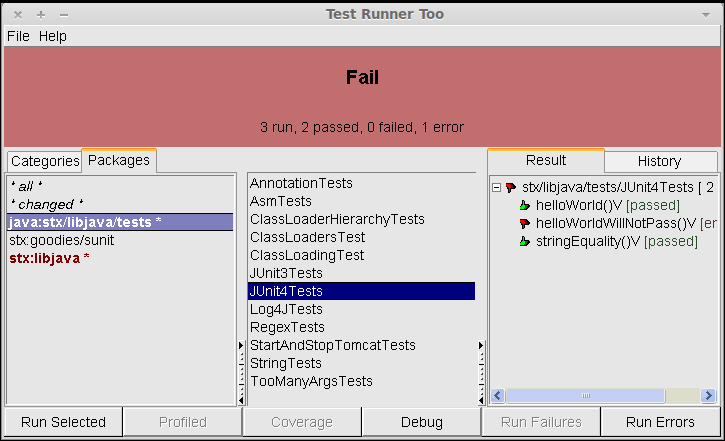
\includegraphics[width=11cm]{figures/test_runner.png}
	\end{center}
	\caption{TestRunner with Java tests loaded}
	\label{fig:test_runner}
\end{figure}

JUnit helped us during implementation of more complex features.
It is integrated into development tools and is well tested and often used.

\section{Groovy}

\href{http://groovy.codehaus.org/}{Groovy} is dynamic language written on top of JVM. 

Its goal is to build upon strength of Java, but also to add dynamic features known from languages such as Python, Ruby or Smalltalk. 

One of its advantages is, that Java syntax is valid also in Groovy. 
That means that all existing Java code is runnable by Groovy.

Groovy introduces many interesting features such as \textbf{Multiple Dispatch} or \textbf{Closures}. 

Groovy is able to compile Groovy code to standard classfile.
This classfile is then executable by normal JVM.

Our motivation to have Groovy running on \libjava{} was based on idea of using Groovy's dynamic features to fill in dynamic nature of Smalltalk/X environment and using Groovy to interpret Java during the Java development.

\textbf{Workspace} in ST/X is a place, where developer can write arbitrary Smalltalk code and evaluate it. 

He can inspect the result of computation, he can just print it or he can just evaluate code and discard return value. 

Because when in IDE, Smalltalk VM is running and one can operate on live objects, workspace is often used during development\footnote{For example calling class methods, setting class variables, testing code, or just tweaking runtime environment by enabling break points, programmatically changing configuration etc.}. 

Workspace is just a normal window with text area, it's the design of Smalltalk, which allows runtime parsing, compilation and execution.

Groovy has similar possibilities, so Groovy evaluator has been integrated into workspace \ref{fig:java_workspace}. 

\begin{figure}[ht]
	\begin{center}
		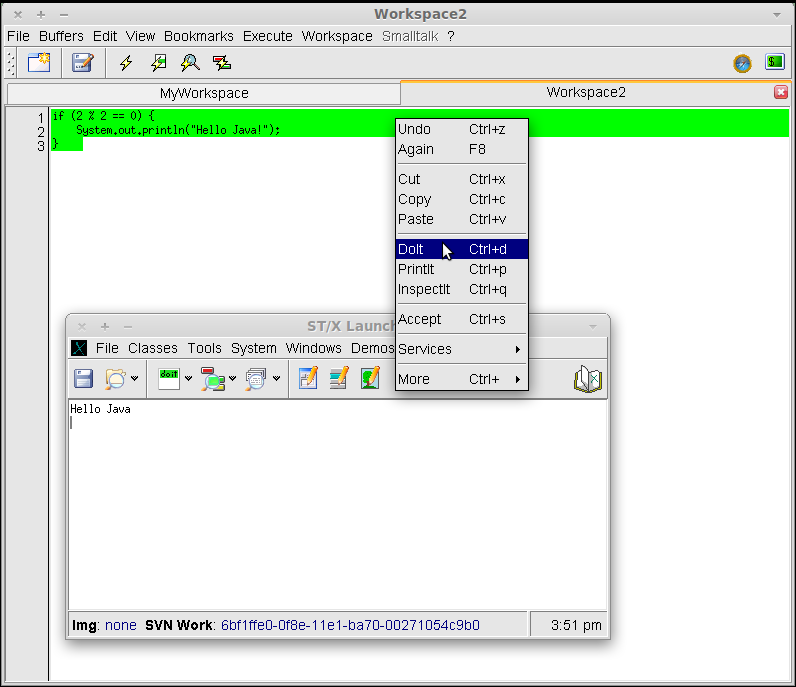
\includegraphics[width=11cm]{figures/java_workspace.png}
	\end{center}
	\caption{Integration of Groovy into Workspace}
	\label{fig:java_workspace}
\end{figure}

It's possible to enter arbitrary Java code, and it gets evaluated. On the Figure \ref{fig:java_workspace} simple code (seen in Listing \ref{code:java_in_groovy}).

\begin{lstlisting}[language=Java, caption=Java code executed by Groovy Workspace, label=code:java_in_groovy]
if (2 % 2 = 0) {
	System.out.println(``Hello Java'');
}
\end{lstlisting} 

Groovy uses various Java features thoroughly, especially reflection and class loaders and helped us to fix many bugs and misunderstandings. 
Arbitrary Java (Groovy) code can be executed in workspace, and this is the first step of having Smalltalk-like development environment for Java.

Work to be done in integration of Groovy into ST/X is for example extending SystemBrowser to be able to accept Java code.
ECJ is probably better suited for this goal though.

\section{ECJ}

\href{http://eclipse.org/jdt/}{ECJ} is part of development tools used in \href{www.eclipse.org}{Eclipse} IDE.
We are able to compile Java class, and it is currently evaluated for use as a part of incremental compiler infrastructure for \libjava{}.

\section{Tomcat}

\href{http://tomcat.apache.org/}{Tomcat} is open source implementation of Java Servlet and JavaServer Pages technologies.
We are able to start the server, we can deploy web applications to it and access them in the web browser.

\begin{figure}[h]
	\begin{center}
		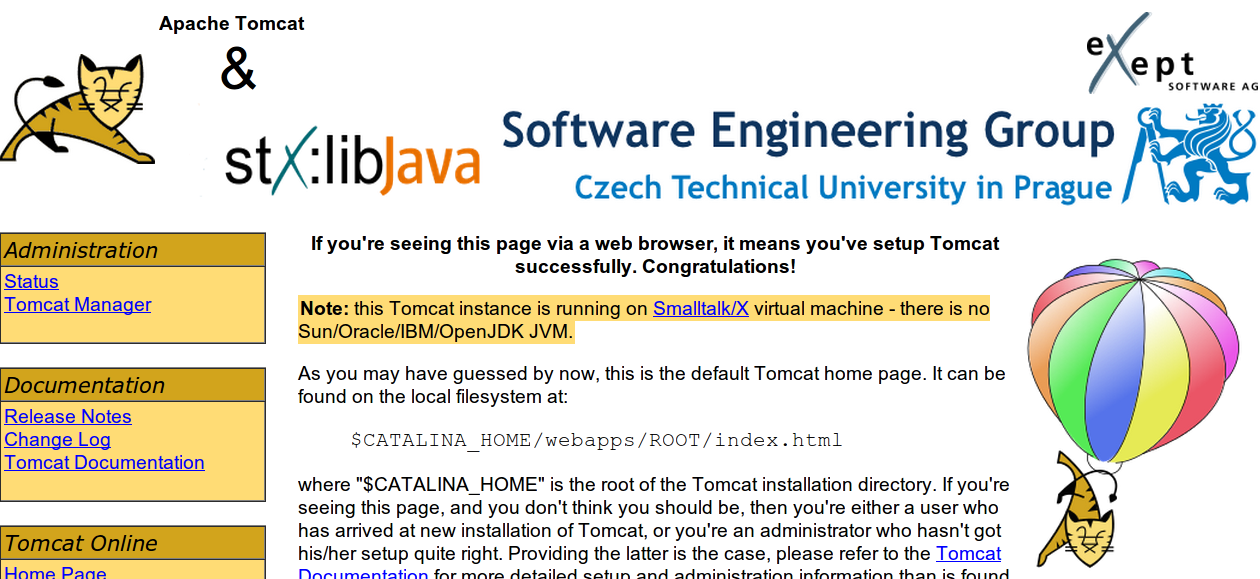
\includegraphics[width=15cm]{figures/tomcat.png}
	\end{center}
	\caption{Screenshot of Tomcat running on the \libjava{}}
	\label{fig:tomcat}
\end{figure}

On the Figure \ref{fig:tomcat}, a slightly modified web application distributed with Tomcat, is running.
This page is accessible from the Internet and a crawler visits links on the website, to test, if our virtual machine is stable enough.
Tomcat is big success as it uses every feature Java language has, it heavily depends on threads and synchronization, it uses class loaders to sandbox web applications, it uses reflection for hot deploy (adding a web application without having to restart the server).
It is even possible to deploy a web application using manager web application (another web application distributed with Tomcat, which serves as remote administration tool).

Making Tomcat work was very demanding, many native methods had to be implemented, various bugs in monitors or class loading were discovered and fixed. 

%*****************************************************************************


\chapter{Summary}
\label{chap:summary}

In this thesis we presented \libjava{} after o year of development.
Initial version was analyzed and in many parts fixed or completelly rewritten.
All essential features required to run Java 6 code were added.

Currently, \libjava{} is able to run Java 6 code, and it has been tested against various Java projects, namely JUnit (a testing framework for Java), Groovy (a dynamic programming language that compiles to Java bytecode), ECJ (a Java compiler) and Tomcat (Servlet and JSP container).

From features added or changed the most important are:

\begin{itemize}
	\item fixes in class loader
	\item redesign of Java Constant pool and resolving logic
	\item implemented notion of Class Loader
	\item redesigned Class Space
	\item reimplemented synchronization, Java monitors
	\item changed native method binding mechanism
	\item many native methods implemented
\end{itemize}

To incrementally compile Java classes, Groovy was explored and integrated into the tools (namely Workspace, part of Smalltalk/X IDE, used to execute arbitrary Smalltalk, and now Java code too). 
Arbitrary Java and Groovy (superset of Java) code can be executed from there.

A tool that allows programmers to use Eclipse compiler for Java from Smalltalk IDE is currently under development.

Future work embodies integration of incremental compiler and Just In Time compiler. 

%*****************************************************************************

\bibliographystyle{csplainnat}
\bibliography{reference}
\appendix


%*****************************************************************************

\chapter{List of used abbreviations}

\begin{description}
\item[JVM] Java Virtual Machine
\item[ST/X] Smalltalk/X
\item[JIT] Just-in-time compiler
\item[JAR] Java Archive, standardized zip-like archive format
\item[IDE] Integrated Development Environment
\item[JLS] Java Language Specification
\end{description}
\vdots

%*****************************************************************************
\chapter{Content of attached CD}

Smalltalk/X development environment, prepared for use with Libjava, is attached on a CD.
To start Smalltalk/X, a shell script is attached as well.
After start up, tutorial.st, interactive tutorial for Libjava, can be opened.

Attached CD has following structure:

\begin{verbatim}
.
+-- README.txt
+-- start_stx.sh
+-- stx
|   +-- bin
|   |   +-- stx
|   |   +-- stc
|   +-- lib
+-- stx.tar.bz2
+-- tutorial.st
\end{verbatim}

%*****************************************************************************
\end{document}
